\documentclass[fontsize=12pt,paper=a4,twoside]{scrartcl}

%Befehl um ToDo-Vermerke zu erstellen
%Autor: Stefan Macke
%Quelle: http://blog.stefan-macke.com/2007/04/23/todo-befehl-in-latex/
\newcommand{\todo}[1]{\textbf{\textsc{\textcolor{red}{(TODO: #1)}}}}

\newcommand{\grad}{\ensuremath{^{\circ}} }
\renewcommand{\strut}{\vrule width 0pt height5mm depth2mm}
\usepackage{booktabs}
\usepackage[utf8]{inputenc}
\usepackage[final]{pdfpages}
% obere Seitenränder gestalten können
\usepackage{fancyhdr}
\usepackage{moreverb}
% Graphiken als jpg, png etc. einbinden können
\usepackage{graphicx}
\usepackage{stmaryrd}
% Floats Objekte mit [H] festsetzen
\usepackage{float}
% setzt URL's schön mit \url{http://bla.laber.com/~mypage}
\usepackage{url}
% Externe PDF's einbinden können
\usepackage{pdflscape}
% Verweise innerhalb des Dokuments schick mit " ... auf Seite ... "
% automatisch versehen. Dazu \vref{labelname} benutzen
\usepackage[ngerman]{varioref}
\usepackage[ngerman]{babel}
\usepackage{ngerman}
 %Bibliographie
\usepackage{bibgerm}
% Tabellen
\usepackage{tabularx}
\usepackage{supertabular}
\usepackage[colorlinks=true, pdfstartview=FitV, linkcolor=blue,
            citecolor=blue, urlcolor=blue, hyperfigures=true,
            pdftex=true]{hyperref}
%\usepackage{bookmark}
\usepackage{hyperref}


% Damit Latex nicht zu lange Zeilen produziert:
\sloppy
%Uneinheitlicher unterer Seitenrand:
\raggedbottom

% Kein Erstzeileneinzug beim Absatzanfang
% Sieht aber nur gut aus, wenn man zwischen Absätzen viel Platz einbaut
\setlength{\parindent}{0ex}

% Abstand zwischen zwei Absätzen
\setlength{\parskip}{1ex}

% Seitenränder für Korrekturen verändern
\addtolength{\evensidemargin}{-1cm}
\addtolength{\oddsidemargin}{1cm}

\bibliographystyle{gerapali}

% Lustige Header auf den Seiten
  \pagestyle{fancy}
  \setlength{\headheight}{70.55003pt}
  \fancyhead{}
  \fancyhead[LO,RE]{Software--Projekt 2\\ WiSe 2013/2014
  \\Projektplan}
  \fancyhead[LE,RO]{Seite \thepage\\\slshape \leftmark\\\slshape \rightmark}

% neuer Befehl: \includegraphicstotab[..]{..}
% Verwendung analog wie \includegraphics
\newlength{\myx} % Variable zum Speichern der Bildbreite
\newlength{\myy} % Variable zum Speichern der Bildhöhe
\newcommand\includegraphicstotab[2][\relax]{%
% Abspeichern der Bildabmessungen
\settowidth{\myx}{\includegraphics[{#1}]{#2}}%
\settoheight{\myy}{\includegraphics[{#1}]{#2}}%
% das eigentliche Einfügen
\parbox[c][1.1\myy][c]{\myx}{%
\includegraphics[{#1}]{#2}}%
}% Ende neuer Befehl

%
% Und jetzt geht das Dokument los....
%

\begin{document}

% Lustige Header nur auf dieser Seite
  \thispagestyle{fancy}
  \fancyhead[LO,RE]{ }
  \fancyhead[LE,RO]{Universität Bremen\\FB 3 -- Informatik\\
  Dr. Karsten Hölscher \\Tutor: Dr. Karsten Hölscher}
  \fancyfoot[C]{}

% Start Titelseite
  \vspace{3cm}

  \begin{minipage}[H]{\textwidth}
  \begin{center}
  \bf
  \Large
  Software--Projekt 2 (RE SWP 2014)\\
  \smallskip
  \small
  VAK 03-BA-901.02\\
  \vspace{3cm}
  
  \end{center}
  \end{minipage}
  \begin{minipage}[H]{\textwidth}
  \begin{center}
  \vspace{1cm}
  \bf
  \Large Projektplan\\ 
  \vspace{3ex}
  \small Schibboleth\\
  
 

\includegraphics[width=0.6\textwidth]{Logo.png}\\

 
  \vfill
  \end{center}
  
  \end{minipage}
  \vfill
  \begin{minipage}[H]{\textwidth}
  \begin{center}
  \sf
  \begin{tabular}{lr}
  Patrick Hollatz & phollatz@tzi.de  \\
  Tobias Dellert & tode@tzi.de \\
  Tim Ellhoff & tellhoff@tzi.de \\
  Daniel Pupat & dpupat@tzi.de \\
  Olga Miloevich & halfelv@uni-bremen.de \\  
  Tim Wiechers & tim3@tzi.de \\
  
  \end{tabular}
  \\ ~
  \vspace{2cm}
  \\
  \it Abgabe: 04. Mai. 2014 --- Version 1.0\\ ~
  \end{center}
  \end{minipage}

% Ende Titelseite

% Start Leerseite

\newpage

  \thispagestyle{fancy}
  \fancyhead{}
  \fancyhead[LO,RE]{RE SWP \\  2014
  \\Projektplan}
  \fancyhead[LE,RO]{Seite \thepage\\\slshape \leftmark\\~}
  \fancyfoot{}
  \renewcommand{\headrulewidth}{0.4pt}
  \tableofcontents
  \listoffigures % Abbildungsverzeichnis 
  \listoftables % Tabellenverzeichnis 

\newpage

  \fancyhead[LE,RO]{Seite \thepage\\\slshape \leftmark\\\slshape \rightmark}


%%%%%%%%%%%%%%%%%%%%%%%%%%%%%%%%%%%%%%%%%%%%%%%%%%%%%%%%%%%%%%%%%%%%%%%%
\section*{Version und Änderungsgeschichte}



\begin{tabular}{ccl}
Version & Datum & Änderungen \\
\hline
0.1 & 23.04.2014 & Ziele hinzugefügt.\\
0.1.1 & 23.04.2014 & Ziele vervollständigt\\
0.1.2 & 25.04.2014 & Hauptarbeitsaktivitäten und --produkte hinzugefügt.\\
0.1.3 & 25.04.2014 & Meilensteine eingefügt.\\
0.1.4 & 26.04.2014 & Benötigte Ressourcen -Menschen hinzugefügt.\\
0.1.5 & 26.04.2014 & Ressourcen ergänzt -Hardware und -Räume.\\
0.1.6 & 26.04.2014 & Budget, Kontaktdaten und Mitarbeiter in den Projektplan eingefügt.\\
0.2 & 27.04.2014 &  Produkte, Evolution d. Plans, Defi. und Akronyme hinzugefügt.\\
0.2.1 & 28.04.2014 & Prozessmodell und Organisationsstruktur eingefügt.\\
0.2.2 & 28.04.2014 & Org.grenzen und -schnitst., Verantwortlichkeiten eingefügt.\\
0.3 & 29.04.2013 & Managementprozesse hinzugefügt.\\
0.4 & 30.04.2014 & Sonstige Elemente und Referenzen hinzugefügt.\\
1.0 & 04.05.2014 & Erste veröffentlichte Version. \\
%1.1 & TT.MM.JJJJ & Zeitplanung für die Anforderungsspezifikation hinzugefügt. \\
%1.2 & TT.MM.JJJJ & .... 
\end{tabular}


%%%%%%%%%%%%%%%%%%%%%%%%%%%%%%%%%%%%%%%%%%%%%%%%%%%%%%%%%%%%%%%%%%%%%%%%

\paragraph{Wichtiger Hinweis:} Dieser Projektplan wurde zu einem großen Teil aus verschiedenen Dokumententeilen anderer Projektpläne unserer Gruppenmitglieder aus dem Wintersemester 2013/14 erstellt. Einige Teile wurden komplett übernommen, andere überarbeitet bzw. angepasst. \\
Diese Vereinbarung haben wir in der Kick-Off-Veranstaltung für RE SWP 2014 mit dem Veranstalter Dr. Karsten Hölscher getroffen. \\
An geeigneten Stellen wird darauf auch noch näher hingewiesen (siehe auch Abschnitt \ref{referenzen}).
		
\section{Einleitung (Daniel Pupat)}

Dieses Dokument ist ein Projektplan für das Modul Softwareprojekt2 im Sommersemester 2014 an der Universität Bremen. Der Projektplan entspricht der Struktur ANSI/IEEE Std. 1058.1-1987\footnote{\url{http://ieeexplore.ieee.org/stamp/stamp.jsp?tp=&arnumber=25325&userType=inst}}.

\subsection{Projektübersicht}


\subsubsection{Ziele}

Das Ziel unserer Gruppe ist es, das Softwareprojekt 2 der Universität Bremen zu bestehen. Dies setzt die Einhaltung der Fristen und Termine, eine ausreichende Fertigstellung des Projekts und die Abgabe aller in SWP2 geforderten Dokumente wie Projektplan, Anforderungsspezifikation und Angebot, Architekturbeschreibung, Schnittstellenbeschreibung, Testplan inklusive Blackbox-Tests und ein elektronisch geführtes Berichtsheft voraus. Darüber hinaus wollen wir einen GUI-Prototypen erstellen und den Akzeptanztest bestehen. Ein Quiz-App zu erstellen steht aber im Vordergrund.

Die Quiz-App benötigt eine Website für die Kundin, sowie einen Zugang für mobile Geräte in Form einer App.
 Ziel ist es geforderte Mindestanforderungen, wie in der Kick-off Veranstaltung vorgestellt und eventuell weitergehende Funktionen zu implementieren.

Zu den Mindestanforderungen gehören die Erstellung und Abgabe einer Quiz-App für mobile Geräte und ein Serverprogramm mit Datenbankanbindung. Die App soll später allen Studenten der Universität Bremen zur Verfügung stehen. Zusätzlich soll die Auftraggeberin über eine Website neue Fragen erstellen oder alte bearbeiten oder löschen können.

\subsubsection{Hauptarbeitsaktivitäten und --produkte}

In einem Softwareprojekt wird der Entwicklungsprozess einer Software in verschiedene Phasen unterteilt.\\
Da das Projekt aus verschiedenen Aktivitäten besteht, lassen sich diese Aktivitäten zu Arbeitsprodukten zusammenfügen. Die Folgende Tabelle bietet eine Übersicht der einzelnen Aktivitäten und den daraus resultierenden Arbeitsprodukten. Die Arbeitsprodukte werden im Laufe des Projektes nach und nach abgegeben.\\

\begin{table}[htbp]
\caption{Hauptaktivitäten und --produkte}
\centering
\begin{tabular}{p{7cm}|p{7cm}}
\hline \textbf{Aktivität / Phase} & \textbf{Arbeitsprodukt} \\ \hline
\hline Projektplanung & Projektplan\\
\hline Anforderungsanalyse, Angebotserstellung & Anforderungsspezifikation, Angebot\\
\hline Entwurf (Globale Analyse, Konzeptionelles Modell, Modulblickwinkel, Ausführungsblickwinkel, Codeblickwinkel) & Architekturbeschreibung\\
\hline Erstellen des Testplans, Tests & Testplan, Schnittstellentests\\
\hline Implementierung & lauffähiges Programm\\
\hline Dokumentation & Installationsanweisung/-Skript\\
\hline Auslieferung & Kunde erhält Produkt\\
\hline 
\end{tabular}
\end{table}

\newpage

\subsubsection{Haupt-Meilensteine und grober Zeitplan}\label{meilensteine}

Die Haupt-Meilensteine resultieren aus den jeweiligen Abgabeterminen der einzelnen Dokumente.

\begin{description}
\item[M0 - 23.04.2014] Kick-Off Veranstaltung.

\item[M1 - 24.04.2014] Beginn des Projektes.

\item[M2 - 04.05.2014] Abgabe initialer Projektplan.\\
Jedes Mitglied muss seinen Teil fertig gestellt haben. Anschließend werden alle Einzelteile zusammengeführt und von allen auf Korrektheit geprüft.

\item[M3 - 08.05.2014] Kundengespräch.

\item[M4 - 27.05.2014] Anforderungsspezifikation (Intern). \\
Jedes Mitglied hat seinen Teil der Anforderungsspezifikation fertiggestellt. Anschließend werden die Teile zusammengeführt und von allen auf Korrektheit geprüft.

\item[M5 - 01.06.2014] Abgabe der Anforderungsspezifikation, GUI-Protoyp und Angebot. \\
Meilenstein 4 muss bereits fertig sein. Der GUI-Prototyp muss vollständig entwickelt sein. Abgabe via MEMS.

\item[M6 - 01.07.2014] Architektur- und Schnittstellenbeschreibung, Testplan, Tests (Intern).\\
Jedes Mitglied muss seine Aufgaben erfüllt haben. Teile werden zusammengeführt und kontrolliert. Tests müssen implementiert sein.

\item[M7 - 06.07.2014] Architekturbeschreibung, Testplan und Schnittstellentests fertig.\\
Meilenstein 7 muss bereits erreicht worden sein. Tests wurden lauffähig implementiert. Abgabe via MEMS.

\item[M8 - 28.07-01.08.2014] Akzeptanztest.

\item[M9 - 10.08.2014] Vollständige Abgabe der Dokumente und der Software. \\
Die Software muss lauffähig und vollständig implementiert sein,\\
Abgabe des Build-/Installationsskriptes
\end{description}

\subsubsection{Benötigte Ressourcen}

\begin{itemize}
\item \textbf{Menschliche Ressourcen}

An menschlichen Ressourcen stehen sechs Informatikstudenten der Universität Bremen zur Verfügung. Wir haben als durchschnittliche Arbeitszeit pro Woche und Person einen Aufwand von ca. 17 Stunden für das Projekt errechnet. Dieser Wert ergibt sich folgendermaßen:\\
\newpage Für das Modul Software Projekt 2 gibt es 9CP. 1CP entspricht 30 Semesterwochenstunden. 9 x 30 = 270 Stunden. Da wir 16 Wochen lang an dem Projekt arbeiten werden, ergibt sich ein aufgerundeter Wert von 17 Stunden pro Woche (270 / 16 = 16,875). Unsere Kontaktdaten sind dem Punkt Mitarbeiter im Abschnitt \ref{sec:Mitarbeiter} zu entnehmen.

\item \textbf{Hard-/ und Software}

Jedes unserer Mitglieder ist im Besitz, oder hat Zugriff, auf Computer, die folgenden Anforderungen und Verfügbarkeiten gerecht werden müssen:

\begin{itemize}
\item zum Anfertigen der Dokumente wird ein Textsatzprogramm benötigt (\LaTeX wird bevorzugt).
\item für die Entwicklung der Software müssen Java-Runtime, ein Texteditor und eine Entwicklungsumgebung mit Android-SDK installiert sein.
\item Git wird zum gleichzeitigen Bearbeiten der Dokumente und zum Datenaustausch der Entwickler benötigt.
\end{itemize}

\item \textbf{Räume}

Das Team wird sich während der gesamten Projektlaufzeit regelmäßig in der e0 im MZH treffen. Weitere spezielle Räumlichkeiten werden nicht benötigt, da wir den Kontakt regelmäßig via Skype oder E-Mail gewährleisten.

\end{itemize}

\subsubsection{Budget}

Ein Budget für dieses Projekt in Form von Geld entfällt, da die Software im Rahmen des Moduls Software Projekt 2 entwickelt wird. Wenn wir über 16 Wochen (vom 24.04.2014 bis zum 10.08.2014) an dem Projekt mit 6 Studenten 17 Stunden pro Woche arbeiten, ergibt sich eine Gesamtsumme von 1632 Entwicklerstunden (16 x 6 x 17 = 1632).

Wir entnehmen einer Studie von Gulp \footnote{\url{http://www.gulp.de/presse/pressemitteilungen/marktstudie-freiberufliche-software-entwickler-sind-gefragt.html}} das zwei Drittel der Software-Entwickler zwischen 60 und 80 Euro fordern. Da wir alle Studenten sind und somit noch in der Ausbildung, setzen wir den Stundenlohn für jeden Entwickler bei 40 Euro an. Somit würden sich für den Arbeitsaufwand der Entwicklerstunden Kosten von insgesamt 65.280 Euro ergeben.

\subsubsection{Kontaktdaten des Kunden}

{\em Jacqueline Sprindt\\
	Rektorat der Universität Bremen\\
	(vertreten durch die Pressestelle)\\
}

\newpage

\subsubsection{Mitarbeiter}\label{sec:Mitarbeiter}

In der Folgenden Tabelle \ref{tableMitarbeiter} stehen die Kontaktdaten aller am Projekt Beteiligten. Ihr sind in Folge Nachname, Name, E-Mail und ein Foto des jeweiligen Teammitglieds zu entnehmen.

\begin{table}[htbp]
\caption{Mitarbeiter}
\label{tableMitarbeiter}
\begin{tabular}{|c|c|c|}
\hline 
\textbf{Name} & \textbf{Email} & \textbf{Foto}\\ \hline \hline
Wiechers, Tim & tim3@tzi.de & \includegraphicstotab[scale=0.125]{tim_wiechers.jpg} \\ \hline
Hollatz, Patrick & phollatz@tzi.de & \includegraphicstotab[scale=0.035]{Patrick.png}\\ \hline
Dellert, Tobias & tode@tzi.de & \includegraphicstotab[scale=0.5, angle=90]{Tobias.jpg}\\\hline
Ellhoff, Tim & tellhoff@tzi.de & \includegraphicstotab[scale=0.1]{Tim.png}\\ \hline
Pupat, Daniel & dpupat@tzi.de & \includegraphicstotab[scale=0.35]{daniel.jpg} \\ \hline
Miloevich, Olga & halfelv@uni-bremen.de & \includegraphicstotab[scale=0.2]{olga.jpg} \\ \hline
\end{tabular}
\end{table}

\newpage

\subsection{Auszuliefernde Produkte\\}

Die Tabelle \ref{reqProd} listet alle auszuliefernde Produkte auf die während des gesamten Projektes anfallen werden.

\begin{table}[htbp]
\caption{Auszuliefernde Produkte}
\label{reqProd}
\centering
\begin{tabular}{|p{4cm}|p{8cm}|p{2cm}|}
\hline Datum & Beschreibung & Anzahl\\ \hline
\hline 04.05.2014 & Initialer Projektplan (dieses Dokument) & 1\\
\hline 01.06.2014 & Anforderungsspezifikation & 1\\
\hline 01.06.2014 & GUI-Prototyp & 1\\
\hline 01.06.2014 & Angebot & 1\\
\hline 06.07.2014 & Architekturbeschreibung & 1\\
\hline 06.07.2014 & Schnittstellenbeschreibung & 1\\
\hline 06.07.2014 & Testplan & 1\\
\hline 10.08.2014 & Vollständige Abgabe & 1\\
\hline 
\end{tabular}
\end{table}

\subsection{Evolution des Plans}

Der Projektplan wird über die gesamte Dauer der Entwicklung durch das Team aktualisiert. Die erste absehbare Aktualisierung wird nach dem Kundengespräch am 08.05.2014 durchgeführt. Weitere absehbare Aktualisierungen des Projektplans sind nach den jeweiligen Hauptabgaben vom Entwicklerteam durchzuführen. \\
Aufgrund der stetigen Entwicklung des Systems sind weitere Aktualisierungen abzusehen, vor allem hinsichtlich der Arbeitspakete. Alle Änderungen werden von dem jeweiligen Phasenleiter überwacht und auf Korrektheit geprüft. Als unvorhergesehene Aktualisierungen wären z.B. das Austreten eines Mitglieds aus der Gruppe zu nennen, da dies die meiste Umstrukturierung mit sich zieht. Die Arbeitspakete müssten in dem Fall neu auf die restlichen Teammitglieder aufgeteilt werden, was wiederum der jeweilige Phasenleiter übernimmt.


\subsection{Referenzen (Olga Miloevich)}\label{referenzen}

\subsubsection{Links}
\begin{itemize}

  \item IT-Fachkunde, ISBN: 978-3-8085-3653-7, Kapitel 6.2 Projektmanagement
  \item Koschke, Rainer: Projektplan-Vorlage SWP1, SS 2013
  \item Koschke, Rainer: Planung (Vorlesungsskript), SS 2013
  \item Gruppe ''irgendwiecool'', Projektplan, SWP 2, WS 2012/13
  \item Gruppe ''ICC'', Projektplan, SWP1, SS2013
  \item Gruppe ''Five and a half man'', Projektplan, SWP 1, SS2013
  \item Gruppe ''YNotZoidberg'', Projektplan, SWP2, WS2013/14
  \item Gruppe ''IT\_R3V0LUT10N'' Projektplan, SWP2, WS2013/14
  \item Gruppe ''ZuSpaet'' Projektplan, SWP2, WS2013/14

\item{\url{http://www.eclipse.org/}\\ Die Website von Eclipse.} \item{\url{https://developer.android.com/sdk/index.html}\\ Die Website von Android-SDK}
\item{\url{http://maven.apache.org/}\\ Die Website des Mavenprojekts.}
\item{\url{http://glassfish.java.net/}\\ Die Website von GlassFish.}
\item{\url{http://junit.org/}\\ Die Website des Test-Frameworks JUnit}
\item{\url{http://github.com/}\\ Die Website von GitHub.}
\item{\url{http://www.ganttproject.biz/}\\ Projektseite für Gantt-Diagramme.}
\item{\url{http://www.latex-project.org/}\\ Die Website des Textsatzsystems \LaTeX.}
\item{\url{http://www.oracle.com/technetwork/java/codeconv-138413.html/}\\ Java Coding-Guidlines.}
\item{\url{http://www.gulp.de/presse/pressemitteilungen/marktstudie-freiberufliche-software-entwickler-sind-gefragt.html}\\ Die Website für die Information des durchschnittlichen Lohns für Software-Entwickler.}
\item{\url{https://www.dreamspark.com/}\\Website von Microsoft Dreamspark zum Download von MS Project für die Gantt-Diagrammerstellung.}
\end{itemize}

\subsubsection{Weitere}
\begin{itemize}
\item{Vorlage dieses Dokuments - Stud.IP Software Projekt 2 1-Projektplan-Vorlage.tex}
\item{Hinweise zu diesem Dokument - Stud.IP 1-Hinweise-Abgabe-Projektplan.pdf}
\item{Java Referenz - \url{http://www.oracle.com/technetwork/java/javase/documentation/api-jsp-136079.html}}
\end{itemize}

% mit \nocite kann man Literatur auflisten, die im Text nicht explizit
% erwähnt ist. \nocite{*} zitiert dann das ganze .bib-File
%
% Die Bibliographie erzeugt man indem man erst
%
% pdflatex bericht.tex
% bibtex bericht
% pdflatex bericht.tex
% pdflatex bericht.tex
%
% benutzt
%\nocite{Knudsen1}
%\nocite{*}
%\bibliography{literatur}

% Das renewcommand verhindert dass für die Literatur eine section* angelegt wird.
% auftaucht
{\renewcommand\section[2]{}
\bibliography{referenzen}
}

\newpage

\subsection{Definitionen und Akronyme\\}

\begin{table}[!h]
\caption{Definition und Akronyme}
\centering
\begin{tabular}{p{7cm}|p{7cm}}
\hline Begriff & Bedeutung\\ \hline
\hline Andorid & Betriebssystem und Software-Plattform für mobile Geräte\\
\hline Android-SDK & SDK = Software-Development-Tool\\
\hline Ansi/IEEE & eine festgelegte Norm vom 'Institute of Electrical and Electronics Engineers, ANSI ist die Abkürzung für 'American National Standards Institute'\\
\hline App & Programm, welches auf mobilen Endgeräten läuft\\
\hline Build-/Installationsskript & Anleitung zum Installieren der Software\\
\hline CP & Credit Points, 1CP entspricht 30 Semesterwochenstunden Arbeitsaufwand\\
\hline Doxygen & Schnittstellendokumentationssystem\\
\hline Eclipse & die von uns genutzte Entwicklungsumgebung\\
\hline Git/GitHub & Online-Projekt Hoster zur Verwaltung von Dokumenten und Sourcecode\\
\hline GUI & Grafische Oberfläche, Abkürzung für Graphical User Interface\\
\hline Java & Java ist eine Programmiersprache\\
\hline JUnit & Framework zum Testen von Java-Programmen\\
\hline \LaTeX & Ein Textsatzprogramm\\
\hline Maven & Projektkompilierungssystem\\
\hline MEMS & Ein elektronisches Abgabesystem der Universität Bremen\\
\hline Server & Ein dauerhaft erreichbarer Rechner, der einen Dienst bereitstellt\\
\hline Skype & Online Kommunikations-Tool\\
\hline Wasserfallmodell & Ein lineares Vorgehensmodell der Softwareentwicklung\\ 
\hline
\end{tabular}
\end{table}

\newpage

\section{Projektorganisation (Daniel Pupat)}

\subsection{Prozessmodell}
\label{sec:prozessmodell}

Das von uns verwendete Wasserfallmodell gliedert die einzelnen Phasen sequentiell aufeinanderfolgend:\\
\begin{itemize}
\item Anforderungsspezifikation
\item Architekturbeschreibung (Entwurf)
\item Implementierung
\item Test
\item Dokumentation
\item Auslieferung
\end{itemize}
In unserem Fall werden sich die Phasen Implementierung, Test und Dokumentation überschneiden um eine effiziente Arbeitsweise zu gewährleisten. Zudem werden wir bereits vor der Implementierung Black-Box-Tests anfertigen.

\subsection{Organisationsstruktur}

Unsere Dateien werden im uns zur Verfügung gestellten Git-Repository gespeichert.\\
Die Kommunikation findet über E-Mail und über Skype statt. Da eines unserer Mitglieder am Wochenende kein Internetzugang hat, muss notfalls Kontakt per Handy aufgenommen werden. \\ 
Zudem werden wir uns wöchentlich in der e0 im MZH treffen. Der genaue Tag dafür steht noch nicht fest.\\ 
Für das Projekt haben wir einen Projektleiter, welcher für die allgemeine Leitung und Organisation des Projekts zuständig ist und einen Kontroller, welcher die Arbeit des Projektleiters überprüft. Für die einzelnen Arbeitspakete haben wir jeweils einen Phasenleiter bestimmt. Dieser ist für die vollständige und rechtzeitige Bearbeitung sowie für die Qualitätssicherung der Abgaben zuständig. Näheres dazu ist im Abschnitt Managementprozess zu finden.

\newpage
\subsection{Organisationsgrenzen und --schnittstellen}

Bei dem Arbeitgeber und der übergeordneten Organisation handelt es sich um zwei verschiedene Parteien, da es sich bei dem Auftraggeber um einen echten Kunden handelt.

{\em \textbf{Auftraggeber:}\\
	Jacqueline Sprindt\\
	Rektorat der Universität Bremen\\
	(vertreten durch die Pressestelle)\\
}

{\em \textbf{Übergeordnete Organisation:}\\ 
	Dr. Karsten Hölscher\\
	Büro: ECO5 (TAB) 2.56\\
    Telefon: +49 (421) 218 64475 \\
    Fax: +49 (421) 218 4322 \\
	E-Mail: hoelsch@uni-bremen.de 
}



\subsection{Verantwortlichkeiten}
\begin{tabular}{|l|l|}
\hline
\textbf{Mitarbeiter} & \textbf{Rolle} \\
\hline
Tobias Dellert & Projektleiter \\
 & Phasenleiter Projektplan \\
\hline
Daniel Pupat & Controller \\
& Phasenleiter  Anforderungsspezifikation \\ 
\hline
Olga Miloevich & Phasenleiterin Architekturbeschreibung \\
\hline
Tim Ellhoff & Phasenleiter Implementierung \\
\hline
Patrick Hollatz & Phasenleiter Testplan \\
\hline
Tim Wiechers & Phasenleiter Präsentation\\
\hline
\end{tabular} \\

Weitere Verantwortlichkeiten, die von jeweils einem Teammitglied während des gesamten Projektzeitraumes besetzt werden müssen, sind Qualitätsmanagement und Risikomanagement.
Die Aufgaben des Qualitätsmanagers sind es, die Qualität aller Bearbeitungen der Teammitglieder sicherzustellen.
Zu den Aufgaben des Risikomanagers gehören das frühzeitige Erkennen von möglichen Problemen und diese präventiv zu vermeiden oder einzudämmen, indem er z.B. Arbeitspakete umverteilt oder andere Lösungen findet. Siehe Abschnitt \ref{riskmanagement}.

%%%%%%%%%%%%%%%%%%%%%%%%%%%%%%%%%%%%%%%%%%%%%%%%%%%%%%%%%%%%%%%%%%%%%%%%

\newpage
\section{Managementprozess (Olga Miloevich, Tim Wiechers)}

\subsection{Managementprozess und --prioritäten}

\textit{Folgender Abschnitt w"urde vom Projektplan von der Gruppe YNotZoidberg (Vorlesung Software Projekt 2, WiSe2013/14 übernommen.}\\

F"ur die Organisation unseres Projektes haben wir einen Projektleiter gew"ahlt.\\
Wir haben zudem die Gruppe in einzelne Arbeitsgruppen eingeteilt. Daf"ur haben wir nach einem schnellen dynamischen System aus der Wirtschaft gesucht und haben das sogenannte Mehrliniensystem ausgew"ahlt. Dieses Mehrliniensystem ist im Gegensatz zur Matrixorganisation oder dem Einzelliniensystem am besten f"ur unsere Umst"ande und Zwecke geeignet. Das System passt am besten f"ur kleine Gruppen, wie unsere. Es lassen sich mehrere Personen zu einer Gruppe zuordnen. \newline
Der Projektmanager "uberwacht den Ablauf des gesamten Projektes und kontrolliert die Arbeitsgruppen. Die Arbeitsgruppen kommunizieren mit den jeweiligen Mitgliedern ihrer Arbeitsgruppe sowie mit allen Gruppenleitern. Bei Bedarf kommunizieren die Arbeiter einer Arbeitsgruppe auch mit Arbeitern anderer Arbeitsgruppen. \\
Die Kommunikationen innerhalb der gesamten Projektgruppen wird durch regelm"a"sige Meetings gew"ahrleistet. Bei Konflikten oder Unstimmigkeiten ist der Projektleiter ein Ansprechpartner und auch Entscheidungstr"ager.\\
Unsere Priorit"ateten liegen bei diesem Projekt haupts"achlich bei der Erf"ullung der Mindestanforderunden in dem gegebenen Zeitraum. Dabei haben wir auch einen Puffer eingeplant. Werden die Mindestanforderunden fr"uhzeitig erf"ullt, dann wird dieser Puffer dazu benutzt, einige Zusatzfunktionen in unsere Software zu integrieren. \\
Unser Budget besteht aus Personen und Personenstunden. Die Planung dieses Budgets "ubernimmt der Projektleiter.\\
Es folgt unser Mehrliniendiagramm.\\
\textit{Quellen: Projektplan von der Gruppe ``Five and a half men'' (Vorlesung Software Projekt 1 2013); Projektplan von der Gruppe ``irgendwiecool'' (Vorlesung Software Projekt 2 2013); Projektplan von der Gruppe ``ICC'' (Vorlesung Software Projekt 1 2013);  Projektplan von der Gruppe ``YNotZoidberg'' (Vorlesung Software Projekt 2 2013/14)}
\newpage
\begin{figure}[h!]
\center{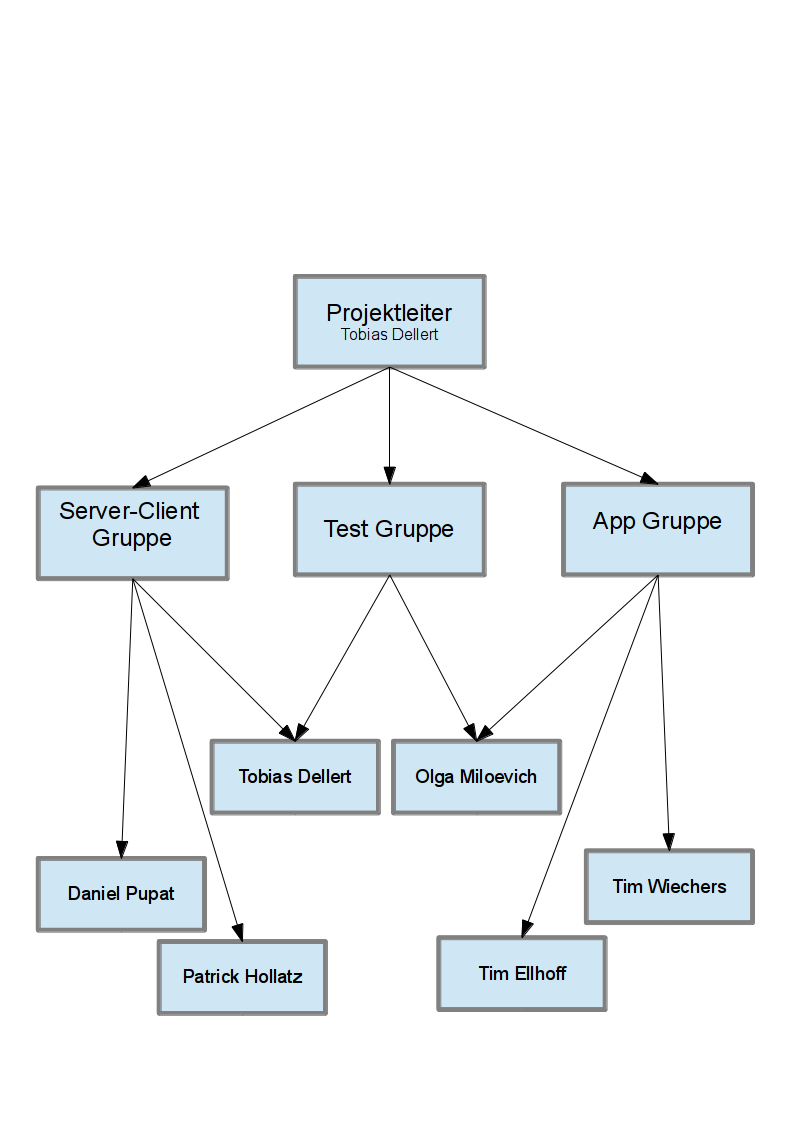
\includegraphics[scale=0.675]{MPGL.png}}
\caption{Mehrliniendiagramm}
\label{Bild:image}
\end{figure}

\newpage
\textit{Folgender Abschnitt w"urde vom Projektplan von der Gruppe IT\_R3V0LUT10N (Vorlesung Software Projekt 2, WiSe2013/14, übernommen.}\\
Die folgenden Managementprozesse haben bei uns die höchsten Prioritäten:
 \\

\underline{Qualität des Produktes:} \\
Unser Ziel ist es, dem Produkt eine hohe Qualität zu geben. Dies ist notwendig, damit der Kunde zufrieden ist und das Produkt später evtl. verwendet wird. Dabei ist wichtig, dass neben den Mindestanforderungen im Idealfall weitere Funktionen vorhanden sind und die Benutzung einfach und benutzerfreundlich ist.\\
Dieses Ziel hat eine hohe Priorität, da dies notwendig ist um den Kunden zufriedenzustellen und eine gute Note zu erreichen.\\
\bigskip \\
\underline{Weiterentwicklung des Produktes:} \\
Es ist auch wichtig, das Produkt so zu entwickeln, damit dieses später bei Bedarf von Anderen weiterentwickelt werden kann. Dies erfordert eine strukturierte Implementierung und ausführliche Dokumentierung.\\
Dieses Ziel hat niedrige Priorität, da wir in erster Linie das Modul bestehen wollen.
\bigskip \\
\underline{Kundenzufriedenheit:}\\
Wir wollen, dass der Kunde später zufrieden ist, was bedeutet, dass man die Mindestanforderungen erfüllt und darüber hinaus noch weitere Features einbindet, da nur so der Kunde wirklich zufrieden ist. \\
Dieses Ziel hat für uns mittlere Priorität, da wir in erster Linie die Mindestanforderungen schaffen wollen und nur wenn noch Zeit ist, weitere Features einbinden. Dies könnte aber noch notwendig sein, um eine gute Note zu erreichen.\\
\bigskip \\
\underline{Kommunikation innerhalb der Gruppe:} \\
Ein wichtiger Faktor ist die Kommunikation innerhalb der Gruppe. Wenn man sich nicht abspricht, kann es zu Schwierigkeiten kommen, wenn z.B. ein Gruppenmitglied seinen Teil nicht rechtzeitig schafft und die anderen aber davon ausgehen.\\
Dieses Ziel hat bei uns eine hohe Priorität, da ohne Kommunikation das Projekt mit hoher Wahrscheinlichkeit scheitert.\\
\bigskip \\
\underline{Klima innerhalb der Gruppe:} \\
Ein gutes Gruppenklima heißt, dass innerhalb der Gruppe alle gut miteinander auskommen und es keinen Streit gibt. Außerdem muss man den Anderen vertrauen können, dass sie immer rechtzeitig fertig werden und bei Problemen Bescheid geben.\\
Dies hat ebenfalls eine hohe Priorität, da gerade das Vertrauen und die Zuverlässigkeit sehr wichtig sind, damit alles rechtzeitig fertig wird.
\bigskip \\
\underline{Gute Note:}\\
Ziel dieser Veranstaltung ist für uns das Projekt so gut wie möglich zu bestehen. Dabei sollte jeder sein Bestes geben, damit am Ende das Maximum an Punkten für die Gruppe erreicht wird.\\
Dies hat bei uns eine hohe Priorität, da wir später einen möglichst guten Abschluss haben wollen.
\bigskip \\
\underline{Kunde entscheidet sich für unser Produkt:}\\
Da der Kunde am Ende der Veranstaltung ein Produkt aussuchen wird, welches dann in der Universität verwendet wird, wäre es möglich, dass er unser Produkt wählt.\\
Dieses Ziel hat bei uns eine niedrige Priorität, da wir in erster Linie gut abschneiden wollen, aber nicht darauf hinarbeiten, unbedingt das beste Produkt der Veranstaltung zu entwickeln, da dies zu zeitaufwendig wäre.


\subsection{Annahmen, Abhängigkeiten und Einschränkungen}
\textit{Folgender Abschnitt w"urde vom Projektplan von der Gruppe IT\_R3V0LUT10N (Vorlesung Software Projekt 2, WiSe2013/14, übernommen.}\\
\subsubsection{Annahmen}
\underline{Mindestanforderungen werden nicht verändert:} \\
Die erste Annahme ist, dass der Kunde die Mindestanforderungen nicht verändert. Dies bedeutet, dass es keine Möglichkeit gibt, andere Mindestanforderungen auszuhandeln und der Kunde auch keine neuen stellt.\\
\bigskip \\
\underline{Deadline wird nicht verschoben:} \\
Noch eine Annahme ist, dass sich die Deadlines der verschiedenen Abgaben unter normalen Umständen nicht verändern. Dies bedeutet, dass der Kunde diese nicht vorverlegt und wir diese nicht nach hinten verlegen können. \\
\bigskip \\
\underline{Erfolgreiche Teilnahme:} \\
Eine weitere Annahme ist, dass alle Gruppenmitglieder die Veranstaltung erfolgreich bestehen wollen. Da sich alle für dieses Modul eingetragen haben, kann man davon ausgehen, dass alle ihr Bestes geben, um diese Veranstaltung zu bestehen.\\
\bigskip \\
\underline{Grundkenntnisse in Java:} \\
Man kann auch annehmen, dass alle Mitglieder Grundkenntnisse in Java haben, da alle Gruppenmitglieder bereits die Veranstaltungen Praktische Informatik 1 und 2 besucht haben.\\

\subsubsection{Abhängigkeiten}

\underline{Laptop:} \\
Da jeder von uns ein Laptop besitzt, werden wir diesen hauptsächlich verwenden, da so jeder mobil ist und überall weiterarbeiten kann.\\
\bigskip \\
\underline{GitHub:} \\
Zum Teilen der Dokumente verwenden wir GitHub. So kann jede Person einen Teil bearbeiten und die Dokumente können dann zusammengeführt werden. \\
\bigskip \\
\underline{Mitglieder:} \\
Da dies eine Gruppenarbeit ist, muss jedes Gruppenmitglied seinen Teil leisten, da die Arbeit auf sechs Leute ausgelegt ist. \\
\bigskip \\
Von den eben genannten Punkten ist das Projekt abhängig, da bei einem Ausfall der Punkte Schwierigkeiten auftreten können.

\subsubsection{Einschränkungen}
\underline{Weitere belegte Module:} \\
Jeder von uns belegt noch weitere Module und hat deswegen nur eine gewisse Zeit für SWP2. Hinzu kommt noch, dass wir Mitglieder haben, die in unterschiedlichen Semestern sind, wodurch es schwierig ist, einen gemeinsamen Termin zu finden. \\

\underline{Deadlines:} \\
Weiterer zeitliche Einschränkung ist bedingt durch die festgelegten Zeitpunkte der einzelnen Abgaben.

\newpage
\subsection{Risikomanagement}\label{riskmanagement}
\textit{Folgender Abschnitt w"urde vom Projektplan von der Gruppe IT\_R3V0LUT10N (Vorlesung Software Projekt 2, WiSe2013/14, übernommen.}\\
\begin{center}
\begin{tabular}{|c|c|c|c|} \hline 
\textbf{Risiko} & \textbf{EW (1-10)} & \textbf{SH (1-10)} & \textbf{RH}\\ \hline \hline
Krankheitsbedingter Ausfall eines Gruppenmitglieds & 5  & 4 & 20\\ \hline
Krankheitsbedingter Ausfall mehrerer Gruppenmitglieder & 2  & 7 & 14\\ \hline
Austritt eines Gruppenmitglieds & 4 & 5 & 20\\ \hline
Austritt mehrerer Gruppenmitglieder & 1 & 8 & 8\\ \hline
Inkompetenz eines Gruppenmitglieds & 2 & 7 & 14\\ \hline
Mangelhafte Kommunikation innerhalb der Gruppe & 4 & 6 & 24\\ \hline
Auflösung/Teilung der Gruppe & 2 & 10 & 20\\ \hline
Unstimmigkeiten in der Gruppe & 2 & 5 & 10\\ \hline
Mangelnde Motivation in der Gruppe & 6 & 5 & 30\\ \hline
Zeitmangel & 6 & 6 & 36\\ \hline
Probleme mit neuen Technologien & 5 & 3 & 15\\ \hline
Ausfall von GitHub & 1 & 8 & 8\\ \hline
Ausfall des Glassfish-servers & 1 & 8 & 8\\ \hline
Mindestanforderung des Kunden falsch interpretiert & 3 & 9 & 27\\ \hline
Fehler in Architekturbeschreibung & 3 & 7 & 21\\ \hline
Ausfall des Rechners eines Gruppenmitglieds & 2 & 7 & 14\\ \hline
Arbeitsfortschritt geht verloren & 2 & 5 & 10\\ \hline
\end{tabular}
\end{center}
EW = Eintrittswahrscheinlichkeit(Skala 1:gering - 10:hoch)\\
SH = Schadenshöhe (Skala 1:gering - 10:hoch)\\
RH = Risikohöhe (EW * SH)\\

\bigskip 

\textbf{\underline{Krankheitsbedingter Ausfall eines/mehrerer Gruppenmitglieds/er:}}\\
Aufgrund von Krankheiten fallen eine oder mehrere Personen aus und können nicht mehr richtig oder für eine gewisse Zeit überhaupt nicht mehr mitarbeiten. Dadurch kommt auf die restliche Gruppe mehr Arbeit zu.\\
\textbf{Maßnahmen zur Schadensbegrenzung:}\\
1. Gruppenmitglied benachrichtigt die anderen Mitglieder so früh wie möglich, damit diese sich darauf einstellen können.\\
2. Die Gruppe sucht Gespräch mit dem Tutor, wenn mehrere Personen ausfallen.\\

\bigskip 

\textbf{\underline{Austritt eines/mehrerer Gruppenmitglieds/er:}}\\
Aufgrund von Zeitmangel, Studienabbruch und anderen Gründen kann es jederzeit passieren, dass Gruppenmitglieder aus der Gruppe austreten. Dadurch müssen die anderen Personen dann entsprechend mehr arbeiten, was zu Problemen führen kann.\\
\textbf{Maßnahmen zur Vorbeugung:}\\
1. Im Zeitplan vor den Deadlines immer ein wenig Zeit überlassen, um durch einen plötzlichen Austritt die Abgabe noch rechtzeitig zu schaffen.\\
\textbf{Maßnahmen zur Schadensbegrenzung:}\\
2. Bei einem Austritt aus der Gruppe gibt das Mitglied den anderen sofort Bescheid, damit diese sich rechtzeitig auf die Mehrarbeit einstellen können.\\
3. Sollten mehrere Mitglieder austreten, Gespräch mit dem Tutor suchen um gegebenenfalls die Anforderungen zu senken.\\

\bigskip 

\textbf{\underline{Inkompetenz eines Gruppenmitglieds:}}\\
Es kann passieren das ein Gruppenmitglied Inkompetent ist und somit nicht in der Lage die ihm zugeteilten Aufgaben zu lösen. Das kann daran liegen, dass dieses Mitglied im bisherigen Studienverlauf immer durch andere Gruppenmitglieder die Module bestanden hat. Dabei kann es passieren, dass dieses Unentdeckt bleibt und so erst spät festgestellt wird das ein Teil nicht funktioniert.\\
\textbf{Maßnahmen zur Schadensbegrenzung:}\\
1. Durch wöchentliche Treffen wird der Fortschritt besprochen und wenn jemand dieses nicht hinbekommt, wird dieses frühzeitig erkannt und der Teil kann unter den anderen Mitgliedern aufgeteilt werden.\\
2. Jedes Gruppenmitglied sollte sich bei Problemen frühzeitig an die Gruppe wenden, damit die anderen diesen helfen können. \\
3. Wenn dieses Gruppenmitglied zu einer Belastung für die Gruppe wird, kann durch eine Gruppenentscheidung dieses Mitglied aus der Gruppe ausgeschlossen werden. \\

\bigskip

\textbf{\underline{Mangelhafte Kommunikation innerhalb der Gruppe:}}\\
Da wir in einer relativ großen Gruppe arbeiten, wird die Arbeit aufgeteilt. Dabei sind viele Teilaufgaben abhängig von anderen, was dazu führen kann, dass ohne Kommunikation die Teilaufgaben oder Implementierungen nicht zusammenpassen. Dadurch kann es im späteren Verlauf zu großen Problemen kommen, da so die Software evtl. nicht läuft.\\
\textbf{Maßnahmen zur Vorbeugung:}\\
1. Die Mitglieder, die stark voneinander abhängige Aufgaben haben, sollte sich vorher genau absprechen und auch die ganze Zeit in Kontakt bleiben, um Missverständnisse zu vermeiden.\\
2. In den wöchentlichen Treffen jede Aufgabe ansprechen, damit jeder weiß, was ungefähr die anderen Mitglieder wie machen.\\
\textbf{Maßnahmen zur Schadensbegrenzung:}\\
3. Jeder sollte sich die Aufgaben der anderen Mitglieder immer durchlesen und gerade bei abhängigen Aufgabenteilen genau drauf achten, dass diese zusammenpassen.\\

\bigskip

\textbf{\underline{Teilung der Gruppe:}}\\
Wenn es Probleme oder Unstimmigkeiten innerhalb der Gruppe gibt und sich zwei Lager bilden, kann es dazu führen, dass sich die Gruppe trennen muss. Dies kann auch passieren, wenn sich herausstellen sollte, dass die Mitglieder starke unterschiedliche Fähigkeiten besitzen und so die besseren Personen die Hauptarbeit verrichten müssen und diese damit nicht einverstanden sind.\\
\textbf{Maßnahmen zur Vorbeugung:}\\
1. Bei unterschiedlichen Fähigkeiten früh festlegen, dass diese später bessere Noten bekommen, damit diese auch zufrieden sind.\\
\textbf{Maßnahmen zur Schadensbegrenzung:}\\
2. Bei Problemen und Unstimmigkeiten das Gespräch suchen und diese Ansprechen und gegebenfalls auch den Tutor hinzuziehen, um die Probleme zu lösen.\\

\bigskip

\textbf{\underline{Auflösung der Gruppe:}}\\
Es kann durch schlechte Abgaben, Zeitmangel, Unstimmigkeiten und Gruppenaustritten eine Gruppenauflösung geben, was zu einem nicht bestehen des Moduls führen würde, da man alleine dieses wahrscheinlich nicht hinbekommen würde. \\
\textbf{Maßnahmen zur Vorbeugung:}
1. Bei Problemen frühzeitig das Gespräch suchen, um zu verhindern, dass sich die Gruppe auflöst.\\

\bigskip

\textbf{\underline{Unzuverlässigkeit eines Gruppenmitglieds:}}\\
Wenn ein Gruppenmitglied seine Aufgaben nicht zu dem geplanten Zeitpunkt fertig bekommt, da er keine Zeit hatte oder andere Prioritäten gesetzt hat, kann es dazu führen, dass die Abgabe nicht vollständig ist und es eine 5.0 für die Abgabe gibt.\\
\textbf{Maßnahmen zur Vorbeugung:}\\
1. Bei der Planung der Zeit immer ein wenig Luft lassen, damit man noch reagieren kann, falls ein Mitglied seine Aufgaben nicht gemacht hat.\\
\textbf{Maßnahmen zur Schadensbegrenzung:}\\
2. Im wöchentlichen Treffen den Fortschritt jedes Mitglieds begutachten und evtl. darauf reagieren, sollte ein Mitglied nicht im Zeitplan sein.\\
3. Mitglied, wenn es die Aufgaben nicht macht beim ersten Mal ermahnen und bei wiederholten Male aus der Gruppe  ausschließen.\\

\bigskip

\textbf{\underline{Unstimmigkeiten in der Gruppe:}}\\
Da sich in der Gruppe Leute befinden, die sich vorher nicht kannten, kann es passieren, dass sich Mitglieder mit anderen Mitgliedern nicht verstehen und so das Gruppenklima stören.\\
\textbf{Maßnahmen zur Schadensbegrenzung:}\\
1. Bei einem Problem, müssen die anderen Gruppenmitglieder schlichten und z.B die Probleme in einem Gruppentreffen ansprechen und lösen.\\

\bigskip 

\textbf{\underline{Mangelnde Motivation in der Gruppe:}}\\
Da SWP 2 sehr zeitaufwendig ist und sich Abgaben über mehrere Wochen erstrecken, kann es gerade am Anfang einer neuen Abgabe zu Mangelnder Motivation kommen, da man denkt, dass man noch genug Zeit hat.\\
\textbf{Maßnahmen zur Vorbeugung:}\\
1. Treffen mit der Gruppe planen, ohne am Projekt zu arbeiten, um die Moral der Gruppe zu stärken und sich gegenseitig zu motivieren.\\

\bigskip

\textbf{\underline{Zeitmangel:}}\\
Da es feste Deadlines für die einzelnen Abgaben gibt, kann es zu Zeitproblemen kommen. Auch durch Ausfälle von Mitgliedern oder schlechte Zeiteinplanung kann es zu zeitlichen Mangel kommen.\\
\textbf{Maßnahmen zur Vorbeugung:}\\
1. Bei der Planung immer einen Zeitpuffer lassen, damit man noch vor den Abgaben Luft hat falls es irgendwelche Probleme während der Bearbeitungsphase gibt.\\
2. Bei den wöchentlichen Treffen immer überprüfen, ob jeder im Zeitplan ist, um notfalls noch früh genug auf Zeitprobleme zu reagieren.\\
\textbf{Maßnahmen zur Schadensbegrenzung:}\\
3. Wenn ein Aufgabenteil in Zeitverzug kommt, diesen auf mehreren Mitgliedern aufteilen, damit dieser noch rechtzeitig fertig wird.\\

\bigskip

\textbf{\underline{Probleme mit neuen Technologien:}}\\
Da wir mit Technologien arbeiten müssen, mit denen wir noch keine oder nur wenig Erfahrung haben wie z.B. Android, kann dies zu unerwarteten Problemen führen. Dadurch kann sich der zeitliche Aufwand stark erhöhen.\\
\textbf{Maßnahmen zur Vorbeugung:}\\
1. Im Zeitplan bereits Zeit zur Einarbeitung neuer Programme einplanen, damit es noch genug Zeit zur Bearbeitung gibt.\\
2. Vorher die Mitglieder so aufteilen, dass die Personen die bereits Erfahrung mit den jeweiligen Technologien haben, diese Aufgabenteile übernehmen.\\
\textbf{Maßnahmen zur Schadensbegrenzung:}\\
3. Falls ein Gruppenmitglied mit einer Technologie überhaupt nicht zurecht kommt, können die Aufgaben mit einem anderen Mitglied getauscht werden.\\

\bigskip

\textbf{\underline{Ausfall von GitHub}}\\
Wir benutzen GitHub als Repository. Es kann passieren, dass es Probleme mit dem Server gibt, was bei uns zu organisatorischen Problemen führen kann.
\textbf{Maßnahmen zur Vorbeugung:}\\
1. Jeder sollte regelmäßig Back-ups durchführen, damit man sichergehen kann, dass keine Daten bei einem Serverabsturz verloren gehen.\\
\textbf{Maßnahmen zur Schadensbegrenzung:}\\
2. Bei einem Server Ausfall werden dem Phasenleiter alle Dokumente per E-Mail geschickt, damit dieser diese zusammenfügen und abschicken kann.\\

\bigskip 

\textbf{\underline{Mindestanforderung des Kunden falsch interpretiert:}}\\
Da es viele Forderungen des Kunden gibt, kann es sein, dass eine falsch verstanden oder vergessen wird und das zu einem nicht bestehen führen würde.\\
\textbf{Maßnahmen zur Vorbeugung:}\\
1. Jedes Mitglied sollte vor der Abgabe für sich alleine noch einmal alle Anforderungen überprüfen und bei zweifeln die Gruppe informieren.\\
2. Bei unklaren Forderungen im Kundengespräch bereits konkrete Fragen dazu stellen.\\

\bigskip

\textbf{\underline{Fehler in Architekturbeschreibung:}}\\
Es kann passieren, dass man in der Architekturbeschreibung bereits Fehler eingebaut hat, die dann später bei der Implementierung entdeckt werden. Dadurch können große Probleme auftreten, gerade wenn man versucht 2 Code Stücke zusammenzufügen.\\
\textbf{Maßnahmen zur Vorbeugung:}\\
1. Bei der Architekturbeschreibung konzentriert arbeiten und sich Zeit lassen für Klassendiagramme etc., damit dort möglichst keine Fehler auftreten.\\
\textbf{Maßnahmen zur Schadensbegrenzung:}\\
2. Sollte jemanden ein Fehler auffallen, der mehrere Komponenten betrifft, sollte dieser möglichst schnell mit der ganzen Gruppe gelöst werden.\\ 

\textbf{\underline{Ausfall des Rechners eines Gruppenmitglieds:}}\\
Ohne einen Rechner kann nicht effektiv am Projekt mitgearbeitet werden. Ein Ausfall ist demnach ein Risiko, bei dem dringend ein Ersatz gefunden werden muss.\\
\textbf{Maßnahmen zur Vorbeugung:}\\
1. Verantwortungsbewusster Umgang und Vorsicht im Zeitraum des Projekts.\\
\textbf{Maßnahmen zur Schadensbegrenzung:}\\
2. Als Alternative kann man auf die Rechner der Uni Bremen ausweichen und büßt so nur Mobilität ein.\\ 

\textbf{\underline{Arbeitsfortschritt geht verloren:}}\\
Ein stundenlanges Arbeiten kann durch unvorhersehbare, z.B. technische Probleme verloren gehen.\\
\textbf{Maßnahmen zur Vorbeugung:}\\
1. Häufiges Abspeichern.\\
2. Häufiges \textit{Commiten} der Änderungen ins GitHub-Repository.

\newpage
\textbf{Die Maßnahmen zur Vorbeugung werden über die gesamte Zeit des Projektes angewendet, bei den Maßnahmen zur Schadensbegrenzung nach Eintritt entscheidet der Phasenleiter, welche Maßnahmen getroffen werden.}\\
\bigskip 

Aufgrund der getroffenen Maßnahmen verändern sich die Werte wie folgt:\\
\begin{center}
\begin{tabular}{|c|c|c|c|} \hline
Risiko & NEW (1-10) & NSH (1-10) & NRH\\ \hline
Krankheitsbedingter Ausfall eines Gruppenmitglieds & 5 & 3 & 15\\ \hline
Krankheitsbedingter Ausfall mehrerer Gruppenmitglieder & 2 & 5 & 10\\ \hline
Austritt eines Gruppenmitglieds & 4 & 3 & 12\\ \hline
Austritt mehrerer Gruppenmitglieder & 1 & 6 & 6\\ \hline
Inkompetenz eines Gruppenmitglieds & 1 & 4 & 4\\ \hline
Mangelhafte Kommunikation innerhalb der Gruppe & 3 & 5 & 15\\ \hline
Teilung der Gruppe & 1 & 8 & 8\\ \hline
Auflösung der Gruppe & 1 & 10 & 10\\ \hline
Unzuverlässigkeit eines Gruppenmitglieds & 2 & 7 & 14\\ \hline
Unstimmigkeiten in der Gruppe & 1 & 5 & 5\\ \hline
Mangelnde Motivation in der Gruppe & 5 & 5 & 25\\ \hline
Zeitmangel & 4 & 5 & 20\\ \hline
Probleme mit neuen Technologien & 4 & 2 & 8\\ \hline
Ausfall von GitHub & 1 & 6 & 6\\ \hline
Ausfall des Glassfish-servers & 1 & 8 & 8\\ \hline
Mindestanforderung des Kunden falsch interpretiert & 2 & 9 & 18\\ \hline
Fehler in Architekturbeschreibung & 3 & 5 & 15\\ \hline
Ausfall des Rechners eines Gruppenmitglieds & 2 & 2 & 4\\ \hline
Arbeitsfortschritt geht verloren & 2 & 3 & 6\\ \hline
\end{tabular}
\end{center}

NEW = Neue Eintrittswahrscheinlichkeit(Skala 1:gering - 10:hoch)\\
NSH = Neue Schadenshöhe (Skala 1:gering - 10:hoch)\\
NRH = Neue Risikohöhe (NEW * NSH)\\


\subsection{Projektüberwachung}\label{3.4-controlling}

Um das Projekt zu überwachen, wird wöchentlich ein Treffen stattfinden, wo überprüft wird, wie weit jeder ist. Später, wenn die Aufgaben stark voneinander abhängig sind, sollte es ein weiteres Treffen geben, um sich untereinander besser abzusprechen. Dies wird gerade ab der Architekturplanung wichtig. Außerdem wird es einen permanenten Austausch über Skype geben, indem über Probleme und Anliegen diskutiert wird. Dieser läuft in erster Linie über einen Gruppenchat ab, sollte es aber einmal etwas konkreter werden, wird untereinander telefoniert. \\
Es wird auch für jede Phase einen Phasenleiter geben, der dafür zuständig ist, den Zeitplan im Auge zu behalten. Diesem Phasenleiter muss dann jedes Gruppenmitglied regelmäßig Bescheid geben, wie weit die Teilaufgabe bereits bearbeitet ist. Sollte es Probleme geben, ist die Aufgabe des Phasenleiters das Risiko einzuschätzen und Maßnahmen zu treffen, welche im Punkt Risikomanagement erläutert sind.\\
Bei größeren Problemen kann ein Treffen spontan einberufen werden oder es wird direkt bei Skype angesprochen und da versucht, dies zu lösen.

\subsection{Mitarbeiter}

Die Mitarbeiter sollten ausreichend Programmierkenntnisse in Java besitzen, damit diese später auch in der Lage sind, die Quizsoftware zu entwerfen. Auch sollten diese zumindest an SWP 1 teilgenommen haben, um die Grundkenntnisse zu haben, die Aufgaben zu bearbeiten. \\
Die Mitarbeiter sollten auch in der Lage zu sein im Team zu arbeiten und sich eigenständig in Themengebiete einzuarbeiten. Bei Problemen sollten die Mitarbeiter sich direkt an die Gruppe wenden, damit diese frühzeitig gelöst werden. Außerdem sollten sie genügend Kenntnisse in Deutsch und Englisch haben, um sich in den Sprachen vernünftig ausdrücken zu können. Die Mitarbeiter sollten zudem noch genügend Kenntnisse in Latex haben, sowie SQL Statements erstellen können. 

\subsubsection{Tim Wiechers}

\textbf{Hardskills}
\begin{itemize}
\item{Gute Kenntnisse in Java.}
\item{Sehr gute Deutsch-/ und Englischkenntnisse}
\item{SQL-Statementerstellung}
\item{solide \LaTeX.Kenntnisse}
\end{itemize}
\textbf{Softskills}
\begin{itemize}
\item{Selbstorganisation}
\item{Teamfähigkeit}
\item{Hilfsbereitschaft}
\end{itemize}

\subsubsection{Tim Ellhoff}

\textbf{Hardskills}
\begin{itemize}
\item{Gute Kenntnisse in Java.}
\item{Sehr gute Deutsch-/ und Englischkenntnisse}
\item{SQL-Statementerstellung}
\item{solide \LaTeX.Kenntnisse}
\item{Gute Kenntnisse im Grafikdesign}
\end{itemize}
\textbf{Softskills}
\begin{itemize}
\item{Selbstorganisation}
\item{Teamfähigkeit}
\item{Hilfsbereitschaft}
\end{itemize}

\subsubsection{Tobias Dellert}

\textbf{Hardskills}
\begin{itemize}
\item{Gute Kenntnisse in Java.}
\item{Sehr gute Deutsch-/ und Englischkenntnisse}
\item{SQL-Statementerstellung}
\item{solide \LaTeX.Kenntnisse}
\item{Gute Kenntnisse im Grafikdesign}
\end{itemize}
\textbf{Softskills}
\begin{itemize}
\item{Selbstorganisation}
\item{Teamfähigkeit}
\item{Hilfsbereitschaft}
\end{itemize}

\subsubsection{Olga Miloevich}

\textbf{Hardskills}
\begin{itemize}
\item{Gute Kenntnisse in Java.}
\item{Sehr gute Deutsch-/ und Englischkenntnisse}
\item{SQL-Statementerstellung}
\item{solide \LaTeX.Kenntnisse}
\item{Gute Kenntnisse im Grafikdesign}
\end{itemize}
\textbf{Softskills}
\begin{itemize}
\item{Selbstorganisation}
\item{Teamfähigkeit}
\item{Hilfsbereitschaft}
\end{itemize}

\subsubsection{Daniel Pupat}

\textbf{Hardskills}
\begin{itemize}
\item{Gute Kenntnisse in Java.}
\item{Sehr gute Deutsch-/ und Englischkenntnisse}
\item{SQL-Statementerstellung}
\item{solide \LaTeX.Kenntnisse}
\item{Gute Kenntnisse im Grafikdesign}
\end{itemize}
\textbf{Softskills}
\begin{itemize}
\item{Selbstorganisation}
\item{Teamfähigkeit}
\item{Hilfsbereitschaft}
\end{itemize}

\subsubsection{Patrick Hollatz}

\textbf{Hardskills}
\begin{itemize}
\item{Gute Kenntnisse in Java.}
\item{Sehr gute Deutsch-/ und Englischkenntnisse}
\item{SQL-Statementerstellung}
\item{solide \LaTeX.Kenntnisse}
\item{Gute Kenntnisse im Grafikdesign}
\end{itemize}
\textbf{Softskills}
\begin{itemize}
\item{Selbstorganisation}
\item{Teamfähigkeit}
\item{Hilfsbereitschaft}
\end{itemize}



%%%%%%%%%%%%%%%%%%%%%%%%%%%%%%%%%%%%%%%%%%%%%%%%%%%%%%%%%%%%%%%%%%%%%%%%

\section{Technische Prozesse (Patrick Hollatz)}
\subsection{Methoden, Werkzeuge und Techniken}
\subsubsection{Entwicklungsplattform}
Zur Erstellung und Verwaltung der einzelnen Dateien, nutzen wir die IDE "`Eclipse Kepler"' \footnote{\url{http://www.eclipse.org/}}.\\
%Mithilfe des Plug-ins "`Android Developer Tools"' in der Version 1.0.0.\_8-7ScKtmH6E8McIScJXJXcITh9wdNni4 können wir direkt in der IDE für Android Software entwickeln. \cite{android}\\
UML-Diagramme erstellen wir mit "`Dia"' Version 0.97.2 \footnote{\url{https://wiki.gnome.org/Apps/Dia}}.\\
Die Dokumenten-Erstellung erfolgt mithilfe von Latex \footnote{\url{http://www.latex-project.org/}}.\\
Um von überall auf unsere Dateien zugreifen zu können, nutzen wir ein Git-Repository bei "`GitHub"' \footnote{\url{http://github.com/}}.\\
Für die komplexe Zeitplanung erstellen wir mithilfe von "`Microsoft Project"' ein Gantt-Diagramm \footnote{\url{http://office.microsoft.com/de-de/projekt-und-portfolioverwaltung-microsoft-project-FX103472268.aspx}}.

\subsubsection{Entwicklungsmethode}

Unsere Entwicklungsmethode ist das Wasserfallmodell, wie in \ref{sec:prozessmodell} vorgestellt. Dabei wird nicht alles sequentiell abgearbeitet, sondern die Phasen Implementierung, Test und Dokumentation werden sich überschneiden.

\subsubsection{Programmiersprache und Bibliotheken}

Die Software wird mit Java auf Basis des "`Java SE Development Kit (JDK) 7"' entwickelt \footnote{\url{http://www.java.com/}}.\\
%Zudem benutzen wir eine leichtgewichtige SQLite-Datenbank, welche wir mithilfe des von Oracle bereitgestellten "`java.sql"' Paketes verwenden können. \cite{database}\\

\subsection{Dokumentationsplan}
Wir werden als Ergebnis verschiedene Dokumentationen vorweisen können. Diese sind:

\begin{itemize}
\item{Nutzerhandbuch}
\item{Installationsanleitung}
\item{Dokumentation des Quellcodes}
\end{itemize}

\subsubsection{Codingstyle}
Unsere Implementierungen werden sich an die \emph{Code Conventions for the Java Programming Language}\footnote{\url{http://www.oracle.com/technetwork/java/codeconv-138413.html}} halten.\\
Unsere .tex Dateien gehen aus der Vorlage für das SWP2-Projekt hervor. Es ist dafür zu sorgen, dass es jederzeit kompilierbar ist.


\subsubsection{Kommentarsprache}

Die Kommentare werden in Englisch geschrieben, um Probleme mit Sonderzeichen zu vermeiden und das Verständnis des Source Codes, bei der Wartung oder Weiterentwicklung, auch nicht deutschsprachigen zu erleichtern bzw. zu ermöglichen.

\subsubsection{JavaDoc}

JavaDoc Kommentare werden für alle öffentlichen Klassen, Methoden und Variablen auf Englisch verfasst, und dienen der Übersicht und schnellerem Verstehen der Zusammenhänge des Projekts.
Private Klassen, Methoden und Variablen werden nur mit JavaDoc Kommentaren versehen, wenn diese Komplex oder für das Verständnis wesentlich sind.

\subsubsection{Begleitende Dokumentation}

Begleitend werden eine Installationsanleitung für die Anwendung und den Server, ein Benutzerhandbuch zur Bedienung und eine Testprotokoll zum schnellen Überblick über durchgeführte Test und deren Ergebnis geschrieben.

\subsection{Unterstützende Projektfunktionen}
%{\em Wie wird Euer Konfigurationsmanagement funktionieren? Wer ist verantwortlich? Benötigt Ihr dazu Ressourcen oder Zeit? Hier könnte z.B.\ der Pfad zum Repository angegeben werden. Plant Ihr Datensicherung?}

Alle erstellten Java-, SQL- und Latex-Dateien werden im Git Repository gespeichert. Dadurch haben wird nicht nur eine Datensicherung, sondern auch eine Versionskontrolle. Das Repository wird beim ersten Gruppentreffen erstellt und anschließend wird der Pfad zum Repository an dieser Stelle hinzugefügt. Das Repository liegt unter \url{https://github.com/timeathotmail/ReSWP.git} .\\
Zur Qualitätssicherung wird jedes Arbeitspaket nach Fertigstellung auf Erfüllung der Anforderungen überprüft, ob es unseren internen Richtlinien entspricht und wird gegebenenfalls noch einmal vom Qualitäts-Manager für eine Überarbeitung empfohlen. Dafür sind nur wenige Arbeitsstunden vorgesehen, wenn der jeweils zuständige nicht selbst an Arbeitsprodukten arbeitet.

%{\em Gibt es Maßnahmen zur Qualitätssicherung? Wer ist zuständig?
%  Wieviel Zeit ist dafür vorgesehen?}

%%%%%%%%%%%%%%%%%%%%%%%%%%%%%%%%%%%%%%%%%%%%%%%%%%%%%%%%%%%%%%%%%%%%%%%%

\section{Arbeitspakete, Zeitplan und Budget}

\textit{bearbeitet von Tim Ellhoff, Tobias Dellert, Olga Miloevich}

\subsubsection{Annahmen}\label{aps}

Wir gehen von folgenden Annahmen aus: \\
\begin{itemize}
\item jedes Mitglied der Gruppe hat rund 14,5 Stunden Zeit in der Woche für das Projekt, davon ausgehend, dass die Veranstaltung SWP2 9CP bringt, was 270 Stunden an Zeit entspricht (1CP = 30 Stunden). Diesen Wert aufgesplittet in 19 Wochen ergibt rechnerisch 14,21 Stunden, also aufgerundet 14,5 Stunden pro Mitglied.

\item eine Arbeitswoche hat 5 Tage, wobei jeder Arbeitstag 8 Arbeitsstunden hat.

\item des Weiteren ist von folgenden Feiertagen und Urlaubszeiten auszugehen:
\begin{itemize}
\item Tag der Arbeit: 01.05.2014
\item Himmelfahrt: 29.05.2014
\item Pfingstmontag: 09.06.2014
\end{itemize}
\end{itemize}
\subsubsection{Anmerkungen}\label{aps}

\paragraph{Hinweis:} \textit{Wir haben die Punkte 'Arbeitspakete', 'Zeitplan und Abhängigkeiten' sowie 'Ressourcenanforderung' zu einem Unterpunkt zusammengefasst.}\\

Wir haben bisher nur die Phasen 'Projektplan' und 'Anforderungsspezifikation' vollständig in den Arbeitspaketen und Zuteilungen behandelt. Die übrigen Phasen des Projekts - Entwurf, Implementierung und Test - können zu diesem Zeitpunkt noch nicht detailliert beschrieben werden, sondern erfolgen stattdessen in grobem Format. \\

\paragraph{Hinweis zum Tabellenlayout:}Da wir in diesem Projektplan Inhalte aus anderen Projektplänen vorheriger SWP-Veranstaltungen z.T. übernehmen (wie mit dem Veranstalter abgesprochen), unterscheidet sich die äußere Form der Arbeitspaket-Tabellen manchmal. 

\subsection{Arbeitspakete, Zeitplan, Abhängigkeiten u. Ressourcenanforderungen}\label{aps}

Im Folgenden liefert eine grafische Übersicht in Form eines Gantt-Diagramms die grundlegenden Arbeitspakete (Abbildung \ref{Gantt-Ueberblick2}).\\

\begin{figure}[!h]
\caption{Gantt-Ueberblick}
%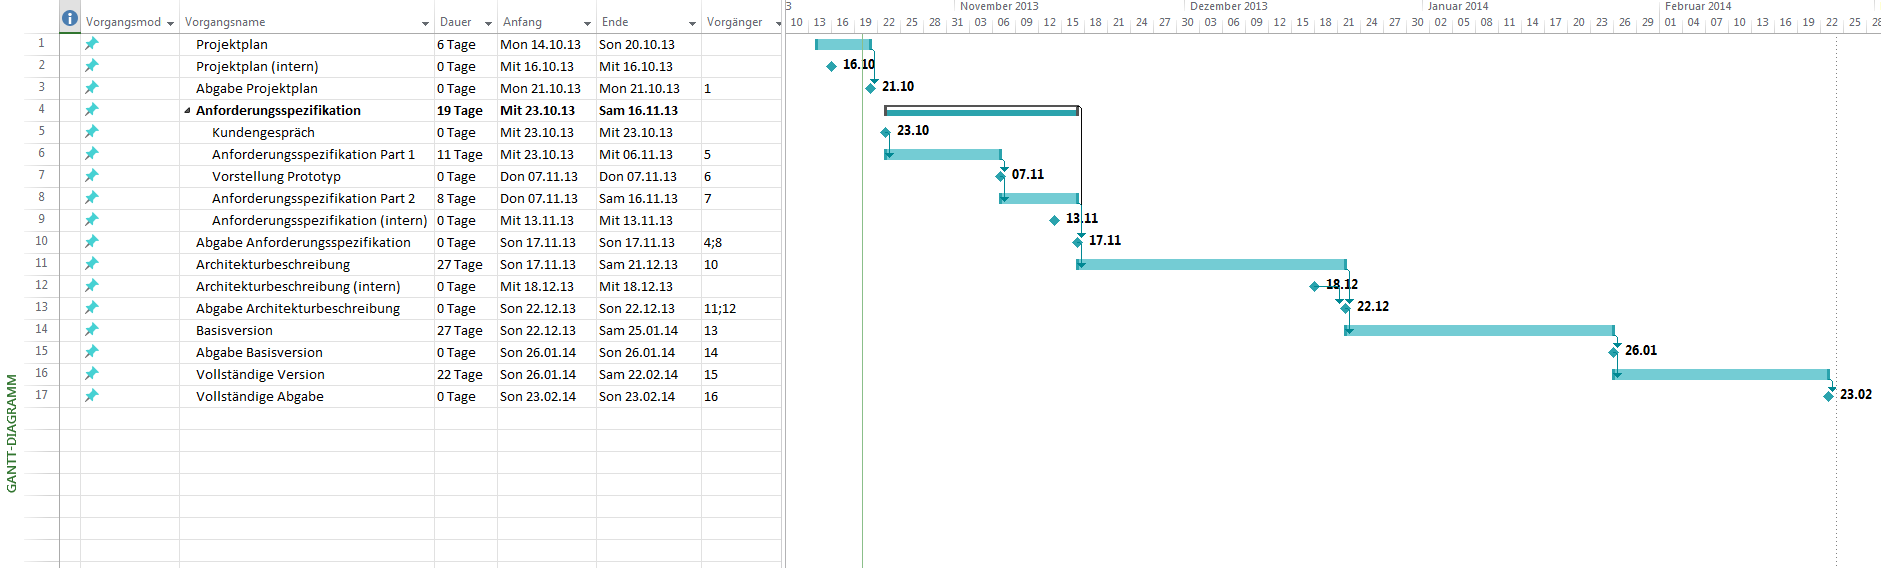
\includegraphics[angle = 90, scale=0.4]{gantt-ueberblick2.png}
\label{Gantt-Ueberblick}
\end{figure}

\newpage

\paragraph{Hinweise zu den Begriffen in den Tabellen:} \textit{Der Punkt 'Gesamtdauer' der jeweiligen Arbeitspakete ist der Zeitbereich zwischen dem Beginn und dem Ende einer bestimmten Aktivität. Der 'Aufwand' ist die tatsächlich aufgewendete Zeit, in der auch gearbeitet wurde. Somit kann die 'Gesamtdauer' häufig höher ausfallen, wenn sich bestimmte Aktivitäten z.B. über Feiertage hinziehen. Mit der 'Abhängigkeit' ist gemeint, ob das Arbeitspaket von anderen abhängig ist, also im Prinzip einen Vorgänger hat. Mit den 'Ressourcen' sind stets Akteure unserer Gruppe gemeint. Der Punkt 'Mindestanforderungen' beschreibt gewissermaßen das Minimalziel des Arbeitspakets (Minimalbedingung), die mindestens erfüllt werden muss, damit es fertig ist.}\\

\subsubsection{Projektplan}\label{aps}

In den folgenden Tabellen sind die Arbeitspakete des Abschnitts 'Projektplan' dargestellt. Grafisch sind diese in einem weiteren Gantt-Diagramm realisiert (Abbildung \ref{Gantt-Projektplan2}). \\

\begin{figure}[htbp]
\caption{Gantt-Projektplan}
%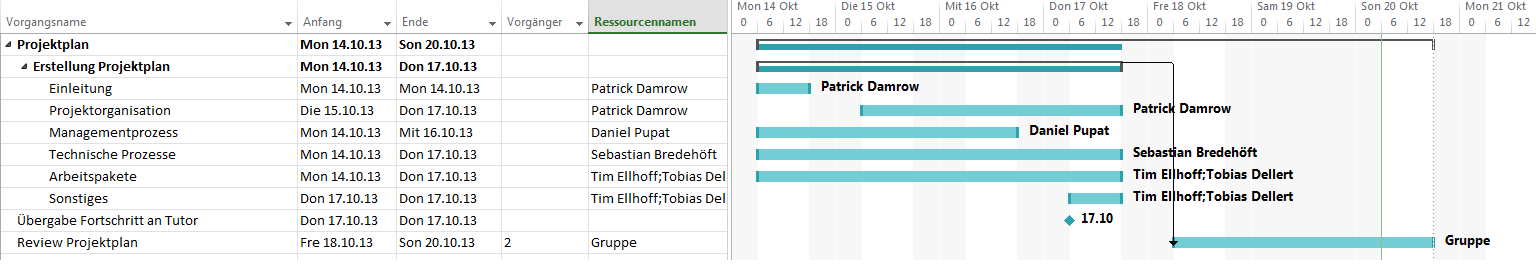
\includegraphics[angle= 90, scale=0.56]{Gantt-Projektplan2.png}

\label{Gantt-Projektplan2}
\end{figure}

\textit{Folgender Abschnitt w"urde vom Projektplan von der Gruppe IT\_R3V0LUT10N (Vorlesung Software Projekt 2, WiSe2013/14, teils übernommen und überarbeitet.}


\begin{tabular}{p{7.5cm}|p{7.5cm}}\toprule
\multicolumn{2}{c}{\textbf{\textit{A R B E I T S P A K E T \quad 1}}} \\ \toprule \hline
\textbf{Bezeichnung} & Gesamter Projektplan\\\hline
\multicolumn{2}{p{15cm}}{\textbf{Beschreibung:} \newline 
Anfertigung und Komplettierung des initalen Projektplans. Details erfolgen in den jeweiligen Unterpunkten.}  \\\hline
\textbf{Hauptverantwortlicher} & Tim Ellhoff\\\hline
\textbf{Abhängigkeit} & -\\\hline
\textbf{Ressourcen} & -\\\hline
\textbf{Aufwand, Gesamtdauer} & \\\hline
\textbf{Beginn} & 22.04.2014 \\\hline
\textbf{Ende} & 04.05.2014\\\hline
\multicolumn{2}{p{15cm}}{\textbf{Mindestanforderungen: } \newline
Die Fertigstellung des initialen Projektplans ist erfolgt und wird durch das interne Gruppen-Review von allen Gruppenmitgliedern überprüft und abgesegnet (Qualitätssicherung).}  \\ \toprule
\end{tabular} \\\\

\begin{tabular}{p{7.5cm}|p{7.5cm}}\toprule
\multicolumn{2}{c}{\textbf{\textit{A R B E I T S P A K E T \quad 1.1}}} \\ \toprule \hline
\textbf{Bezeichnung} & Projektplanerstellung\\\hline
\multicolumn{2}{p{15cm}}{\textbf{Beschreibung:} \newline 
siehe Unterpunkte}  \\\hline
\textbf{Hauptverantwortlicher} & Tobias Dellert und Tim Ellhoff\\\hline
\textbf{Abhängigkeit} & -\\\hline
\textbf{Ressourcen} & -\\\hline
\textbf{Aufwand, Gesamtdauer} & \\\hline
\textbf{Beginn} & 27.04.2014 \\\hline
\textbf{Ende} & 03.05.2014\\\hline
\multicolumn{2}{p{15cm}}{\textbf{Mindestanforderungen: } \newline
Die Unterpunkte des Projektplans wurden abgearbeitet und der Projektplan kann im Gruppenreview überprüft werden.}  \\ \toprule
\end{tabular} \\\\

\begin{tabular}{p{7.5cm}|p{7.5cm}}\toprule
\multicolumn{2}{c}{\textbf{\textit{A R B E I T S P A K E T \quad 1.1.1}}} \\ \toprule \hline
\textbf{Bezeichnung} & Einleitung\\\hline
\multicolumn{2}{p{15cm}}{\textbf{Beschreibung:} \newline 
\textit{Erledigung des Projektplanteils:} Die Projektübersicht liefert die Ziele, Hauptarbeitsaktivitäten und -produkte, die Hauptmeilensteine und einen groben Zeitplan, die Erfassung der Ressourcen, die zur Verfügung stehenden Budgets sowie die Kontaktdaten des Kunden und Informationen über die Mitarbeiter am Projekt. Des Weiteren beinhaltet die Einleitung eine Übersicht der auszuliefernden  Produkte mit Terminangaben , sowie Informationen über die Evolution des Plans und die Festlegung von Definitionen bzw. Akronymen.}  \\\hline
\textbf{Hauptverantwortlicher} & Daniel Pupat\\\hline
\textbf{Abhängigkeit} & -\\\hline
\textbf{Ressourcen} & \begin{itemize}
\itemsep0pt
\item Daniel Pupat
\end{itemize} \\\hline
\textbf{Aufwand, Gesamtdauer} & \\\hline
\textbf{Beginn} & 25.04.2014 \\\hline
\textbf{Ende} & 26.04.2014\\\hline
\multicolumn{2}{p{15cm}}{\textbf{Mindestanforderungen: } \newline
Sobald der Projektplanteil fertig ist, kann er zum Gruppenreview weitergegeben werden. }  \\ \toprule
\end{tabular} \\\\

\begin{tabular}{p{7.5cm}|p{7.5cm}}\toprule
\multicolumn{2}{c}{\textbf{\textit{A R B E I T S P A K E T \quad 1.1.2}}} \\ \toprule \hline
\textbf{Bezeichnung} & Projektorganisation\\\hline
\multicolumn{2}{p{15cm}}{\textbf{Beschreibung:} \newline 
\textit{Erledigung des Projektplanteils:} In diesem Abschnitt wird das verwendete Prozessmodell beschrieben, die Organisationsstruktur festgelegt (insbes. Pflichten der Gruppenmitglieder, Kommunikationswege, wöchentliche Treffen usw.), Informationen zu den Organisationsschnittstellen wie Auftraggeber und Arbeitgeber gegeben und letztlich die Verantwortlichkeiten im Projekt festgelegt und unter den einzelnen Gruppenmitgliedern aufgeteilt.    }  \\\hline
\textbf{Hauptverantwortlicher} & Olga Miloevich\\\hline
\textbf{Abhängigkeit} & -\\\hline
\textbf{Ressourcen} & \begin{itemize}
\itemsep0pt
\item Olga Miloevich
\end{itemize} \\\hline
\textbf{Aufwand, Gesamtdauer} & \\\hline
\textbf{Beginn} & 28.04.2014 \\\hline
\textbf{Ende} & 30.04.2014\\\hline
\multicolumn{2}{p{15cm}}{\textbf{Mindestanforderungen: } \newline
Sobald der Projektplanteil fertig ist, kann er zum Gruppenreview weitergegeben werden. }  \\ \toprule
\end{tabular} \\\\

\begin{tabular}{p{7.5cm}|p{7.5cm}}\toprule
\multicolumn{2}{c}{\textbf{\textit{A R B E I T S P A K E T \quad 1.1.3}}} \\ \toprule \hline
\textbf{Bezeichnung} & Managementprozess\\\hline
\multicolumn{2}{p{15cm}}{\textbf{Beschreibung:} \newline 
\textit{Erledigung des Projektplanteils:} Im Managementprozess erfolgt die Festlegung der Managementprozesse (insbes. Ziele des Projekts), sowie die Einhaltung von gewissen Regeln im Punkt 'Annahmen', die eine Vereinbarung der Abhängigkeiten, an denen das Projekt unmittelbar geknüpft ist und die Erfassung von Einschränkungen, die berücksichtigt werden müssen, mit einschließt. Es folgen Angaben zum Risikomanagement (insbes. Ausfall bzw. Austritt von Gruppenmitgliedern, allgemeine Probleme etc.) , Maßnahmen zur Projektüberwachung sowie die Fixierung der Kompetenzen der Mitarbeiter im Projekt.  }  \\\hline
\textbf{Hauptverantwortlicher} & Olga Miloevich\\\hline
\textbf{Abhängigkeit} & -\\\hline
\textbf{Ressourcen} & \begin{itemize}
\itemsep0pt
\item Tim Ellhoff
\end{itemize} \\\hline
\textbf{Aufwand, Gesamtdauer} & \\\hline
\textbf{Beginn} & 27.04.2014 \\\hline
\textbf{Ende} & 29.04.2014\\\hline
\multicolumn{2}{p{15cm}}{\textbf{Mindestanforderungen: } \newline
Sobald der Projektplanteil fertig ist, kann er zum Gruppenreview weitergegeben werden. }  \\ \toprule
\end{tabular} \\\\

\begin{tabular}{p{7.5cm}|p{7.5cm}}\toprule
\multicolumn{2}{c}{\textbf{\textit{A R B E I T S P A K E T \quad 1.1.4}}} \\ \toprule \hline
\textbf{Bezeichnung} & Technische Prozesse\\\hline
\multicolumn{2}{p{15cm}}{\textbf{Beschreibung:} \newline 
\textit{Erledigung des Projektplanteils:} In diesem Abschnitt erfolgt die Festlegung der Entwicklungsplattformen, -methoden und der verwendeten Programmiersprache, sowie eine Vereinbarung über die Eckpfeiler der im Laufe es Projekts abzugebenden Dokumentationen. Unterstützende Projektfunktionen wie die Ernennung von Phasenleitern und die Verwendung eines Versionskontrollsystems nebst Datensicherungen wird schließlich vereinbart. }  \\\hline
\textbf{Hauptverantwortlicher} & Patrick Hollatz \\\hline
\textbf{Abhängigkeit} & -\\\hline
\textbf{Ressourcen} & \begin{itemize}
\itemsep0pt
\item Patrick Hollatz
\end{itemize} \\\hline
\textbf{Aufwand, Gesamtdauer} & \\\hline
\textbf{Beginn} & 29.04.2014 \\\hline
\textbf{Ende} & 29.04.2014\\\hline
\multicolumn{2}{p{15cm}}{\textbf{Mindestanforderungen: } \newline
Sobald der Projektplanteil fertig ist, kann er zum Gruppenreview weitergegeben werden. }  \\ \toprule
\end{tabular} \\\\

\begin{tabular}{p{7.5cm}|p{7.5cm}}\toprule
\multicolumn{2}{c}{\textbf{\textit{A R B E I T S P A K E T \quad 1.1.5}}} \\ \toprule \hline
\textbf{Bezeichnung} & Arbeitspakete, Zeitplan u. Budget\\\hline
\multicolumn{2}{p{15cm}}{\textbf{Beschreibung:} \newline 
\textit{Erledigung des Projektplanteils:} In diesem Punkt werden die Arbeitspakete aller Projektphasen erarbeitet. Zunächst folgen gewisse Annahmen und Anmerkungen sowie Begrifferklärungen für die Arbeitspakete, bevor dann kleinschrittig die Arbeitspakete in tabellarischer und grafischer Form erfasst werden. Es folgen weitere Arbeitspakete für die Dokumentabgaben, Informationen und Vereinbarungen über Meetings innerhalb der Gruppe und der Festlegung des kritischen Pfads für das Projekt.}  \\\hline
\textbf{Hauptverantwortlicher} & Tobias Dellert, Tim Ellhoff \\\hline
\textbf{Abhängigkeit} & -\\\hline
\textbf{Ressourcen} & \begin{itemize}
\itemsep0pt
\item Tobias Dellert
\item Tim Ellhoff
\item Olga Miloevich
\end{itemize} \\\hline
\textbf{Aufwand, Gesamtdauer} & \\\hline
\textbf{Beginn} & 23.04.2014 \\\hline
\textbf{Ende} & 28.04.2014\\\hline
\multicolumn{2}{p{15cm}}{\textbf{Mindestanforderungen: } \newline
Sobald der Projektplanteil fertig ist, kann er zum Gruppenreview weitergegeben werden. }  \\ \toprule
\end{tabular} \\\\

\begin{tabular}{p{7.5cm}|p{7.5cm}}\toprule
\multicolumn{2}{c}{\textbf{\textit{A R B E I T S P A K E T \quad 1.1.6}}} \\ \toprule \hline
\textbf{Bezeichnung} & Sonstige Elemente\\\hline
\multicolumn{2}{p{15cm}}{\textbf{Beschreibung:} \newline 
\textit{Erledigung des Projektplanteils:} Der Abschnitt 'Sonstiges' liefert Informationen über die Pläne für die Konvertierung von Daten, Management-, Ausbildungs- und Raum- und Installationspläne sowie den Plan über die letztendliche Abgabe bzw. Übergabe des Systems. }  \\\hline
\textbf{Hauptverantwortlicher} & Olga Miloevich \\\hline
\textbf{Abhängigkeit} & -\\\hline
\textbf{Ressourcen} & \begin{itemize} 
\itemsep0pt
\item Tim Ellhoff
\end{itemize} \\\hline
\textbf{Aufwand, Gesamtdauer} & \\\hline
\textbf{Beginn} & 02.05.2014 \\\hline
\textbf{Ende} & 03.05.2014\\\hline
\multicolumn{2}{p{15cm}}{\textbf{Mindestanforderungen: } \newline
Sobald der Projektplanteil fertig ist, kann er zum Gruppenreview weitergegeben werden. }  \\ \toprule
\end{tabular} \\\\

\begin{tabular}{p{7.5cm}|p{7.5cm}}\toprule
\multicolumn{2}{c}{\textbf{\textit{A R B E I T S P A K E T \quad 1.2}}} \\ \toprule \hline
\textbf{Bezeichnung} & Gruppenreview des Projektplans\\\hline
\multicolumn{2}{p{15cm}}{\textbf{Beschreibung:} \newline 
Im internen Gruppenreview wird der fertige Projektplan diskutiert, ggf. verbessert bzw. noch geändert.}  \\\hline
\textbf{Hauptverantwortlicher} & Tobias Dellert, Tim Ellhoff \\\hline
\textbf{Abhängigkeit} & 1 Projektplan, 1.1 Projektplanerstellung\\\hline
\textbf{Ressourcen} & \begin{itemize}
\itemsep0pt
\item Tobias Dellert
\item Tim Ellhoff
\item Tim Wiechers
\item Patrick Hollatz
\item Daniel Pupat
\item Olga Miloevich
\end{itemize} \\\hline
\textbf{Aufwand, Gesamtdauer} & \\\hline
\textbf{Beginn} & 03.05.2014 \\\hline
\textbf{Ende} & 04.05.2014\\\hline
\multicolumn{2}{p{15cm}}{\textbf{Mindestanforderungen: } \newline
Der Projektplan ist nun von allen Gruppenmitgliedern in einem Review noch einmal auf den Prüfstand gestellt worden und ist nun fertig. }  \\ \toprule
\end{tabular} \\\\

\subsubsection{Anforderungsspezifikation}\label{aps}

In den folgenden Tabellen sind die Arbeitspakete des Abschnitts 'Anforderungsspezifikation' dargestellt. Grafisch sind diese in einem weiteren Gantt-Diagramm realisiert.

\textit{Folgender Abschnitt w"urde vom Projektplan von der Gruppe YNotZoidberg (Vorlesung Software Projekt 2, WiSe2013/14, teils übernommen und überarbeitet.}


\textit{Bearbeitet von: Olga Miloevich, Tobias Dellert, Tim Ellhoff}\\

\begin{tabular}{|p{7.43cm}|p{7.43cm}|}
\hline
\textbf{AP Titel: }2. Anforderungsspezifikation & \textbf{AP Nummer:} 1 \\ 
\hline
\textbf{Dauer: } 05.05.14- 29.05.14 & \textbf{Aufwand: }147 Std.\\
\hline
\end{tabular}
\begin{tabular}{|p{15.3cm}|}
\hline
\textbf{AP-Teilnehmer: } alle Mitglieder\\
\hline
\textbf{Beschreibung: }Anfertigung und Komplettierung der Anforderungsspezifikation. Details erfolgen in den jeweiligen Unterpunkten\\
\hline
\textbf{Voraussetzung: }keine \\
\hline 
\textbf{Ziele: }Die Fertigstellung der Anforderungsspezifikation ist erfolgt.\\
\hline 
\end{tabular}
\begin{verbatim}

\end{verbatim}
\begin{tabular}{|p{7.43cm}|p{7.43cm}|}
\hline
\textbf{AP Titel: } 2.0.1 Gruppentreffen & \textbf{AP Nummer:} 2 \\ 
\hline
\textbf{Dauer: }09.05.14-23.05.14 & \textbf{Aufwand: }9 Std.\\
\hline
\end{tabular}
\begin{tabular}{|p{15.3cm}|}
\hline
\textbf{AP-Teilnehmer: } Alle Mitglieder\\
\hline
\textbf{Beschreibung: }Dient als qualitätssichernde Maßnahme,
indem Fortschritte und Unklarheiten in der Gruppe besprochen werden.
Ein bis zweimal wöchentlich werden wir uns in der Universität treffen.\\
\hline
\textbf{Voraussetzung: }keine\\
\hline 
\textbf{Ziele: }Jedes Gruppenmitglied ist auf den aktuellen Stand was Änderungen bzgl. des eigenen Arbeitsfeldes angeht.\\
\hline 
\end{tabular}
\begin{verbatim}

\end{verbatim}
\begin{tabular}{|p{7.43cm}|p{7.43cm}|}
\hline
\textbf{AP Titel: }2.1 GUI-Prototyp & \textbf{AP Nummer: }3 \\ 
\hline
\textbf{Dauer: }08.05.14 - 25.05.14 & \textbf{Aufwand: }48 Std.\\
\hline
\end{tabular}
\begin{tabular}{|p{15.3cm}|}
\hline
\textbf{AP-Teilnehmer: }Tobias Dellert, Olga Miloevich, Patrick Hollatz, Tim Ellhoff, Daniel Pupat\\
\hline
\textbf{Beschreibung: }Dem Kundengespräch folgend, wird dem Kunden erstmal eine Benutzeroberfl"ache vorgestellt.\\
\hline
\textbf{Voraussetzung: }stattgefundenes Kundengespräch\\
\hline 
\textbf{Ziele: }Die Grundfunktionen m"ussen anhand des Prototyps pr"asentierbar sein.\\
\hline 
\end{tabular}
\begin{verbatim}

\end{verbatim}
\begin{tabular}{|p{7.43cm}|p{7.43cm}|}
\hline
\textbf{AP Titel: }2.1.1 Story-Board & \textbf{AP Nummer: }4 \\ 
\hline
\textbf{Dauer: }08.05.14 - 10.05.14 & \textbf{Aufwand: }6 Std.\\
\hline
\end{tabular}
\begin{tabular}{|p{15.3cm}|}
\hline
\textbf{AP-Teilnehmer: }Patrick Hollatz\\
\hline
\textbf{Beschreibung: }\\
\hline
\textbf{Voraussetzung: }Kundengespräch\\
\hline 
\textbf{Ziele: }Mit dem Prototyp lassen sich die Leistungsfaktoren pr"asentieren.\\
\hline 
\end{tabular}
\begin{verbatim}

\end{verbatim}
\begin{tabular}{|p{7.43cm}|p{7.43cm}|}
\hline
\textbf{AP Titel: }2.1.2 Design & \textbf{AP Nummer: }5 \\ 
\hline
\textbf{Dauer: }08.05.14- 10.05.15 & \textbf{Aufwand: }10 Std.\\
\hline
\end{tabular}
\begin{tabular}{|p{15.3cm}|}
\hline
\textbf{AP-Teilnehmer: }Olga Miloevich\\
\hline
\textbf{Beschreibung: }\\
\hline
\textbf{Voraussetzung: }keine\\
\hline 
\textbf{Ziele: }Einzusetzendes Design.\\
\hline 
\end{tabular}
\begin{verbatim}

\end{verbatim}
\begin{tabular}{|p{7.43cm}|p{7.43cm}|}
\hline
\textbf{AP Titel: }2.1.3 Entwicklungsphase I & \textbf{AP Nummer: }6 \\ 
\hline
\textbf{Dauer: }09.05.14 - 15.05.14 & \textbf{Aufwand: }20 Std.\\
\hline
\end{tabular}
\begin{tabular}{|p{15.3cm}|}
\hline
\textbf{AP-Teilnehmer: }Olga Miloevich, Tim Ellhoff, Tobias Dellert\\
\hline
\textbf{Beschreibung: }Entwicklung des GUI-Prototyps.\\
\hline
\textbf{Voraussetzung: }Kundengespräch erfolgt.\\
\hline 
\textbf{Ziele: }Mit dem Prototyp lassen sich die Leistungsfaktoren pr"asentieren.\\
\hline 
\end{tabular}
\begin{verbatim}

\end{verbatim}
\begin{tabular}{|p{7.43cm}|p{7.43cm}|}
\hline
\textbf{AP Titel: }2.1.4 Prototyp-Vorstellung & \textbf{AP Nummer: }7\\ 
\hline
\textbf{Dauer: }xx.05.14 & \textbf{Aufwand: }2 Std.\\
\hline
\end{tabular}
\begin{tabular}{|p{15.3cm}|}
\hline
\textbf{AP-Teilnehmer: }Daniel Pupat, Tobias Dellert\\
\hline
\textbf{Beschreibung: }Vorstellung des GUI-Prototyps für den Kunden. \\
\hline
\textbf{Voraussetzung: }Alle anderen Arbeitspakete zum GUI-Abschnitt.\\
\hline 
\textbf{Ziele: } Vorstellung erfolgt.\\
\hline 
\end{tabular}
\begin{verbatim}

\end{verbatim}
\begin{tabular}{|p{7.43cm}|p{7.43cm}|}
\hline
\textbf{AP Titel: }2.1.5 Entwicklungsphase II & \textbf{AP Nummer: }8 \\ 
\hline
\textbf{Dauer: }18.05.14-24.05.14 & \textbf{Aufwand: }10 Std.\\
\hline
\end{tabular}
\begin{tabular}{|p{15.3cm}|}
\hline
\textbf{AP-Teilnehmer: }Olga Miloevich, Tim Ellhoff\\
\hline
\textbf{Beschreibung: } \\
\hline
\textbf{Voraussetzung: }\\
\hline 
\textbf{Ziele: }\\
\hline 
\end{tabular}
\begin{verbatim}

\end{verbatim}
\begin{tabular}{|p{7.43cm}|p{7.43cm}|}
\hline
\textbf{AP Titel: }2.2 Anforderungsspezifikation Dokument & \textbf{AP Nummer: }9\\ 
\hline
\textbf{Dauer: }05.05.14 - 27.05.14 & \textbf{Aufwand: }90 Std.\\
\hline
\end{tabular}
\begin{tabular}{|p{15.3cm}|}
\hline
\textbf{AP-Teilnehmer: }alle Mitglieder\\
\hline
\textbf{Beschreibung: } Herstellung des PDF-Dokumentes Anforderungsspezifikation.\\
\hline
\textbf{Voraussetzung: }keine. \\
\hline 
\textbf{Ziele: }Der Ist-Zustand ist analysiert und dokumentiert.\\
\hline 
\end{tabular}
\begin{verbatim}

\end{verbatim}
\begin{tabular}{|p{7.43cm}|p{7.43cm}|}
\hline
\textbf{AP Titel: }2.2.1 Einleitung & \textbf{AP Nummer: }10\\ 
\hline
\textbf{Dauer: }10.05.14-11.05.14 & \textbf{Aufwand: }2 Std.\\
\hline
\end{tabular}
\begin{tabular}{|p{15.3cm}|}
\hline
\textbf{AP-Teilnehmer: }Patrick Hollatz\\
\hline
\textbf{Beschreibung: }Erledigung des Projektplanteils. Die Projekt"ubersicht liefert die Ziele, Hauptarbeitsaktivit"aten und -produkte, die Hauptmeilsteine und einen groben Zeitplan, die Erfassung der Ressourcen, die zur Verf"ugung stehenden Budgets sowie die Kontaktdaten des Kunden und Informationen "uber die Mitarbeiter am Projekt. Des Weiteren beinhaltet die Einleitung eine "Ubersicht der auszuliefernden Produke mit Terminangaben, sowie Informationen "uber die Evaluation des Plans und die Festlegung von Definitionen bzw. Akronymen.\\
\hline
\textbf{Voraussetzung: }keine.\\
\hline 
\textbf{Ziele: }Projektplanteil wird zum Gruppenreview weitergegeben.\\
\hline 
\end{tabular}
\begin{verbatim}

\end{verbatim}
\begin{tabular}{|p{7.43cm}|p{7.43cm}|}
\hline
\textbf{AP Titel: }2.2.2 Allgemeine Beschreibungen & \textbf{AP Nummer: }11\\ 
\hline
\textbf{Dauer: }08.05.14-13.05.14 & \textbf{Aufwand: }39 Std.\\
\hline
\end{tabular}
\begin{tabular}{|p{15.3cm}|}
\hline
\textbf{AP-Teilnehmer: }Tim Ellhoff, Tobias Dellert, Daniel Pupat, Patrick Hollatz\\
\hline
\textbf{Beschreibung: }siehe Unterpunkte.\\
\hline
\textbf{Voraussetzung: }\\
\hline 
\textbf{Ziele: }\\
\hline 
\end{tabular}
\begin{verbatim}

\end{verbatim}
\begin{tabular}{|p{7.43cm}|p{7.43cm}|}
\hline
\textbf{AP Titel: }2.2.2.1 Vorgang der Ist-Analyse & \textbf{AP Nummer: }12\\ 
\hline
\textbf{Dauer: }08.05.14-13.05.14 & \textbf{Aufwand: }11 Std.\\
\hline
\end{tabular}
\begin{tabular}{|p{15.3cm}|}
\hline
\textbf{AP-Teilnehmer: }Tobias Dellert, Tim Ellhoff\\
\hline
\textbf{Beschreibung: }siehe Unterpunkte.\\
\hline
\textbf{Voraussetzung: }Kundengesrp"ach erfolgt.\\
\hline 
\textbf{Ziele: }Die Unterpunkte des Kundengespr"achs wurden abgearbeitet, somit ist der Ist-Zustand analysiert und dokumentiert.\\
\hline 
\end{tabular}

\begin{tabular}{|p{7.43cm}|p{7.43cm}|}
\hline
\textbf{AP Titel: }2.2.2.1.1 Analyse "ahnlicher Systeme & \textbf{AP Nummer: }13\\
\textbf{Dauer: }10.05.14-13.05.14 & \textbf{Aufwand: }6 Std.\\
\hline
\end{tabular}
\begin{tabular}{|p{15.3cm}|}
\hline
\textbf{AP-Teilnehmer: }Patrick Hollatz, Daniel Pupat\\
\hline
\textbf{Beschreibung: }Das ermittelte Gesamtbild wird mit "ahnlichen bew"ahrten Softwaresystemen verglichen. Deren Eigenheiten und daraus resultierende Vor- und Nachteile werden erschlossen und die Systeme als Ganzes bewertet.\\
\hline
\textbf{Voraussetzung: }\\
\hline 
\textbf{Ziele: }Analyse "ahnlicher Systeme.\\
\hline 
\end{tabular}

\begin{tabular}{|p{7.43cm}|p{7.43cm}|}
\hline
\textbf{AP Titel: }2.2.2.1.2 Vorbereitung auf Kundengespr"ach & \textbf{AP Nummer: }14\\ 
\hline
\textbf{Dauer: }07.05.14 & \textbf{Aufwand: } 1 Std.\\
\hline
\end{tabular}
\begin{tabular}{|p{15.3cm}|}
\hline
\textbf{AP-Teilnehmer: }Tim Ellhoff, Tobias Dellert\\
\hline
\textbf{Beschreibung: }Um ein effektives, aufschlussreiches Interview zu gew"ahrleisten, ist eine konkrete Vorstellung der zu stellenden Fragen von N"oten. Ziel ist es, nach M"oglichkeit alle Anforderungen und W"unsche des Kunden, sowohl die bewussten, als auch die unbewussten, herauszustellen. Daf"ur wird hier ein Fragenkatalog erstellt, der auf Kunden mit beliebigem Wissenstand "uber technische Details anwendbar ist.\\
\hline
\textbf{Voraussetzung: }keine.\\
\hline 
\textbf{Ziele: }Der entstehende Fragenkatalog muss weitestgehend alle Fragen enthalten, die f"ur genaues Verst"andnis der W"unsche und Anforderungen des Kunden n"otig sind.\\
\hline 
\end{tabular}

\begin{tabular}{|p{7.43cm}|p{7.43cm}|}
\hline
\textbf{AP Titel: } Kundengespräch & \textbf{AP Nummer:} 15 \\ 
\hline
\textbf{Dauer: }08.05.14 & \textbf{Aufwand: }2 Std.\\
\hline
\end{tabular}
\begin{tabular}{|p{15.3cm}|}
\hline
\textbf{AP-Teilnehmer: }Tim Ellhoff, Tobias Dellert\\
\hline
\textbf{Beschreibung: }Gespräch mit dem Kunden um dessen Wünsche und Erwartungen an das Produkt festzustellen.\\
\hline
\textbf{Voraussetzung: }keine\\
\hline 
\textbf{Ziele: }Klarheit über die Anforderungen des Kunden verschaffen.\\
\hline 
\end{tabular}

\begin{tabular}{|p{7.43cm}|p{7.43cm}|}
\hline
\textbf{AP Titel: }2.2.2.1.4 Auswertung des Kundengespr"achs & \textbf{AP Nummer: }16\\ 
\hline
\textbf{Dauer: }08.05.14& \textbf{Aufwand: } 2 Std.\\
\hline
\end{tabular}
\begin{tabular}{|p{15.3cm}|}
\hline
\textbf{AP-Teilnehmer: }alle Mitglieder\\
\hline
\textbf{Beschreibung: }Die erhaltenen Ausk"unfte werden zusammengebracht und zu einem gro"sen Bild aus Anforderungen zusammengef"ugt.\\
\hline
\textbf{Voraussetzung: }Kundengespräch erfolgt.\\
\hline 
\textbf{Ziele: }Das erhaltene Gesamtbild enth"alt alle gegebenen Anforderungen, die nach dem Kundengespräch vom Kunden als Leistungsfaktoren angesehen werden.\\
\hline 
\end{tabular}

\begin{tabular}{|p{7.43cm}|p{7.43cm}|}
\hline
\textbf{AP Titel: }2.2.2.2 Vorgang der Soll-Analyse & \textbf{AP Nummer: }17\\ 
\hline
\textbf{Dauer: }15.05.14 - 19.05.14 & \textbf{Aufwand: } 28 Std.\\
\hline
\end{tabular}
\begin{tabular}{|p{15.3cm}|}
\hline
\textbf{AP-Teilnehmer: }Daniel Pupat, Tim Ellhoff, Patrick Hollatz, Tim Wiechers\\
\hline
\textbf{Beschreibung: }\\
\hline
\textbf{Voraussetzung: }Kundengespräch erfolgt.\\
\hline 
\textbf{Ziele: }\\
\hline 
\end{tabular}

\begin{tabular}{|p{7.43cm}|p{7.43cm}|}
\hline
\textbf{AP Titel: } 2.2.2.2.1 Herausstellen der Produktperspektiven & \textbf{AP Nummer: }18\\ 
\hline
\textbf{Dauer: }15.05.14 - 17.05.14 & \textbf{Aufwand: } 6 Std.\\
\hline
\end{tabular}
\begin{tabular}{|p{15.3cm}|}
\hline
\textbf{AP-Teilnehmer: }Tim Ellhoff, Tim Wiechers\\
\hline
\textbf{Beschreibung: }Hier werden die gegebenen Rahmenbedienungen und M"oglichkeiten analysiert, um die realistische Durchf"uhrung und dessen Aufwand zu erfassen. Beachtet und analysiert werden folgende Bereiche:
\begin{enumerate}
 \item Systemschnittstellen
 \item Benutzerschnittstellen
 \item Hardwareschnittstellen
 \item Softwareschnittstellen
 \item Kommunikationsschnittstellen
 \item Speicherbeschr"ankungen
 \item Betriebsmodi
 \item lokale Anpassungen
\end{enumerate}
\\
\hline
\textbf{Voraussetzung: }Siehe Oberpunkt.\\
\hline 
\textbf{Ziele: } Die in der Beschreibung aufgez"ahlten Punkte k"onnen in der Anforderungsspezifikation eindeutig und exakt beschrieben werden.\\
\hline 
\end{tabular}

\begin{tabular}{|p{7.43cm}|p{7.43cm}|}
\hline
\textbf{AP Titel: }2.2.2.2.2 Anwendungsf"alle & \textbf{AP Nummer: }19\\ 
\hline
\textbf{Dauer: }17.05.14 - 19.05.14 & \textbf{Aufwand: } 8 Std.\\
\hline
\end{tabular}
\begin{tabular}{|p{15.3cm}|}
\hline
\textbf{AP-Teilnehmer: }Daniel Pupat, Patrick Hollatz, Tim Wiechers\\
\hline
\textbf{Beschreibung: }Siehe Unterpunkte.\\
\hline
\textbf{Voraussetzung: }Siehe Oberpunkt.\\
\hline 
\textbf{Ziele: }Anwendungsf"alle aller Grundfunktionen sind erfasst und kurz beschrieben.\\
\hline 
\end{tabular}

\begin{tabular}{|p{7.43cm}|p{7.43cm}|}
\hline
\textbf{AP Titel: }2.2.2.2.2.1 Auflistung der Anwendungsf"alle & \textbf{AP Nummer: }20\\ 
\hline
\textbf{Dauer: }17.05.14 & \textbf{Aufwand: } 3 Std.\\
\hline
\end{tabular}
\begin{tabular}{|p{15.3cm}|}
\hline
\textbf{AP-Teilnehmer: }Patrick Hollatz\\
\hline
\textbf{Beschreibung: }Die einzelnen Anwendungsf"alle werden hier aufgelistet und kurz beschrieben.\\
\hline
\textbf{Voraussetzung: }Kundengespr"ach ausgewertet.\\
\hline 
\textbf{Ziele: }Anwendungsf"alle aller Grundfunktionen sind erfasst und kurz beschrieben.\\
\hline 
\end{tabular}

\begin{tabular}{|p{7.43cm}|p{7.43cm}|}
\hline
\textbf{AP Titel: }2.2.2.2.2 Anwendungs- und Sequenzdiagramme & \textbf{AP Nummer: }21\\ 
\hline
\textbf{Dauer: }18.05.14 - 19.05.14 & \textbf{Aufwand: } 5 Std.\\
\hline
\end{tabular}
\begin{tabular}{|p{15.3cm}|}
\hline
\textbf{AP-Teilnehmer: }Tim Wiechers, Daniel Pupat\\
\hline
\textbf{Beschreibung: }Die Anwendungsf"alle werden passenderweise in Anwendungsdiagramme "ubertragen, wobei bei komplexeren F"allen zum Wohle der "Ubersicht auch Sequenzdiagramme hinzugezogen werden k"onnen.\\
\hline
\textbf{Voraussetzung: }Anwendungsf"alle ausgewertet.\\
\hline 
\textbf{Ziele: }Die Anwendungsf"alle der Grundfunktionen sind in einem Anwendungsfalldiagramm dargestellt.\\
\hline 
\end{tabular}

\begin{tabular}{|p{7.43cm}|p{7.43cm}|}
\hline
\textbf{AP Titel: }2.2.2.2.3 Charakteristika & \textbf{AP Nummer: }22\\ 
\hline
\textbf{Dauer: }18.05.14 & \textbf{Aufwand: } 4 Std.\\
\hline
\end{tabular}
\begin{tabular}{|p{15.3cm}|}
\hline
\textbf{AP-Teilnehmer: }Tim Wiechers\\
\hline
\textbf{Beschreibung: }Sinn dieses Arbeitspakets ist, einen vollständigen Einblick des für uns relevanten Ausschnitts der Realität zu erhalten, um damit in sich geschlossene Strukturen von den einzelnen Akteuren untereinander zu schaffen und damit einen verbesserten Überblick der möglichen Anwendungsfälle zu bekommen. Hierzu werden Benutzerklassen erstellt, die so gut wie möglich die unterschiedlichsten Charaktere, Umstände und Motive abdecken.
\\
\hline
\textbf{Voraussetzung: }\\
\hline 
\textbf{Ziele: }Die entstandenen Persona sind umfassend und untereinander verschieden genug, um alle m"oglichen Anwendungsf"alle in Bezug auf die erforderten Grundfunktionen der Software zu erhalten.
\\
\hline 
\end{tabular}

\begin{tabular}{|p{7.43cm}|p{7.43cm}|}
\hline
\textbf{AP Titel: }2.2.2.2.4 Einschr"ankungen& \textbf{AP Nummer: }23\\ 
\hline
\textbf{Dauer: }17.05.14 - 19.05.14& \textbf{Aufwand: } 6 Std.\\
\hline
\end{tabular}
\begin{tabular}{|p{15.3cm}|}
\hline
\textbf{AP-Teilnehmer: }Patrick Hollatz\\
\hline
\textbf{Beschreibung: }Es werden sowohl technische, als auch gesetzliche Rahmenbedingungen festgelegt. Zus"atzlich sollen sicherheitskritische Aspekte durch genauere Spezifikationen der einzelnen Schnittstellen im vorigen Arbeitspaket 2.2.1 begutachtet werden.\\
\hline
\textbf{Voraussetzung: }Herausstellen der Produktperspektiven.\\
\hline 
\textbf{Ziele: }Die technischen und gesetzlichen Rahmenbedingungen sind eindeutig spezifiziert. Alle sicherheitskritischen Aspekte wurden erfasst.\\
\hline 
\end{tabular}

\begin{tabular}{|p{7.43cm}|p{7.43cm}|}
\hline
\textbf{AP Titel: }2.2.2.2.5 "Uberblick, sowie Ausblick in die Zukunft & \textbf{AP Nummer: }24\\ 
\hline
\textbf{Dauer: }18.05.14 - 19.05.14 & \textbf{Aufwand: } 4 Std.\\
\hline
\end{tabular}
\begin{tabular}{|p{15.3cm}|}
\hline
\textbf{AP-Teilnehmer: }Tim Ellhoff\\
\hline
\textbf{Beschreibung: }"Uberblick der Abh"angigkeiten von projekteigenen Faktoren untereinander, sowie ein Blick in die nahe Zukunft, was Ver"anderungen und Erweiterungen sowohl im technischen und rechtlichen Bereich, sowie im Anwendungsumfeld der zu entwickelnden Software angeht. Die Anforderungen sollen entsprechend ver"ander-
 und anpassbar sein.\\
\hline
\textbf{Voraussetzung: }\\
\hline 
\textbf{Ziele: }Die Abh"angigkeit des Entwicklungs- und Erweiterungsprozess von einzelnen pojekteigenen Faktoren wurden umfassend herausgestellt. Zu erwartende Ver"anderungen in der nahen Zukunft( sofern vorhanden ) wurden dokumentiert.\\
\hline 
\end{tabular}

\begin{tabular}{|p{7.43cm}|p{7.43cm}|}
\hline
\textbf{AP Titel: }2.2.3 Detallierte Beschreibungen & \textbf{AP Nummer: }25\\ 
\hline
\textbf{Dauer: }20.05.14 -25.05.14 & \textbf{Aufwand: } 36 Std.\\
\hline
\end{tabular}
\begin{tabular}{|p{15.3cm}|}
\hline
\textbf{AP-Teilnehmer: }Alle Mitglieder\\
\hline
\textbf{Beschreibung: }\\
\hline
\textbf{Voraussetzung: }Bedingt. Siehe Unterpunkte.\\
\hline 
\textbf{Ziele: } Hier findet der Übergang von allgemeinen Anforderungen zu detaillierteren Anwendungen und Konzepten, die für die Architekturbeschreibung wegweisend sein werden.\\
\hline 
\end{tabular}

\begin{tabular}{|p{7.43cm}|p{7.43cm}|}
\hline
\textbf{AP Titel: }2.2.3.1 Datenmodell & \textbf{AP Nummer: }26\\ 
\hline
\textbf{Dauer: }22.05.14 & \textbf{Aufwand: } 4 Std.\\
\hline
\end{tabular}
\begin{tabular}{|p{15.3cm}|}
\hline
\textbf{AP-Teilnehmer: }Tobias Dellert\\
\hline
\textbf{Beschreibung: }Das zu entwickelnde Datenmodell soll eine konzeptionelle Darstellung von dem Weltausschnitt der Quiz-App, als UML-Diagramm, werden.
\\
\hline
\textbf{Voraussetzung: }Kundengespräch, Gesprächsauswertung.\\
\hline 
\textbf{Ziele: }Die Informationen und deren Beziehungen sind dem Weltausschnitt entsprechend in das Datenmodell gesetzt und es l"asst sich somit als Konzept f"ur sp"atere Spezifizierungen benutzen.\\
\hline 
\end{tabular}

\begin{tabular}{|p{7.43cm}|p{7.43cm}|}
\hline
\textbf{AP Titel: }2.2.3.2 Detallierte Anwendungsf"alle & \textbf{AP Nummer: }27\\ 
\hline
\textbf{Dauer: }21.05.14 - 25.05.14 & \textbf{Aufwand: } 20 Std.\\
\hline
\end{tabular}
\begin{tabular}{|p{15.3cm}|}
\hline
\textbf{AP-Teilnehmer: }Daniel Pupat, Olga Miloevich\\
\hline
\textbf{Beschreibung: }Die bereits aufgelisteten Anwendungsf"alle werden mit den Personas und genaueren Beschreibungen erg"anzt. Das Hineinversetzen in die unterschiedlichen Personas hilft die bisherige Funktionalit"at aus der Sicht der Benutzer zu sehen.\\
\hline
\textbf{Voraussetzung: }\\
\hline 
\textbf{Ziele: }Die Anwendungsfälle müssen insgesamt die ganze gewünschte Funktionalität der Software wiedergeben.\\
\hline 
\end{tabular}

\begin{tabular}{|p{7.43cm}|p{7.43cm}|}
\hline
\textbf{AP Titel: }2.2.3.2.1 Screenshots der Benutzeroberfl"ache & \textbf{AP Nummer: }28\\ 
\hline
\textbf{Dauer: } 23.05.14-24.05.14 & \textbf{Aufwand: } 2 Std.\\
\hline
\end{tabular}
\begin{tabular}{|p{15.3cm}|}
\hline
\textbf{AP-Teilnehmer: }Patrick Hollatz\\
\hline
\textbf{Beschreibung: }Die Screenshots der Benutzeroberfläche werden benutzt, um die spezifischen Anwendungsfälle zu illustrieren. Dazu werden die Screenshots an de passenden Stellen beschriftet.\\
\hline
\textbf{Voraussetzung: }GUI-Prototyp ist fertig.\\
\hline 
\textbf{Ziele: }\\
\hline 
\end{tabular}

\begin{tabular}{|p{7.43cm}|p{7.43cm}|}
\hline
\textbf{AP Titel: }2.2.3.3 Aktionen & \textbf{AP Nummer: }29\\ 
\hline
\textbf{Dauer: }20.05.14 - 23.05.14 & \textbf{Aufwand: } 8 Std.\\
\hline
\end{tabular}
\begin{tabular}{|p{15.3cm}|}
\hline
\textbf{AP-Teilnehmer: }Tim Wiechers\\
\hline
\textbf{Beschreibung: }Die bisher beschriebenen Anwendungsfälle werden noch genauer ausgeführt, sodass jede aufgelistete Aktion eine einzelne Nutzung einer beliebigen Funktion( Knopfdruck, Klick ins Textfeld ) der Software beschreibt\\
\hline
\textbf{Voraussetzung: }Anwendungsfälle\\
\hline 
\textbf{Ziele: }Alle Anwendungsfälle sind in die kleinstmöglichen Aktionen aufgeteilt und geordnet.\\
\hline 
\end{tabular}

\begin{tabular}{|p{7.43cm}|p{7.43cm}|}
\hline
\textbf{AP Titel: }2.2.3.4 Systemattribute & \textbf{AP Nummer: }30\\ 
\hline
\textbf{Dauer: }25.05.14 & \textbf{Aufwand: } 2 Std.\\
\hline
\end{tabular}
\begin{tabular}{|p{15.3cm}|}
\hline
\textbf{AP-Teilnehmer: }Tobias Dellert, Tim Ellhoff\\
\hline
\textbf{Beschreibung: }\\
\hline
\textbf{Voraussetzung: }\\
\hline 
\textbf{Ziele: }Die Informationen und deren Beziehungen sind dem Weltausschnitt entsprechend in das Datenmodell gesetzt und es lässt sich somit als Konzept für spätere Spezifizierungen benutzen.\\
\hline 
\end{tabular}

\begin{tabular}{|p{7.43cm}|p{7.43cm}|}
\hline
\textbf{AP Titel: }2.4 Anforderungsspezifikation komplettieren & \textbf{AP Nummer: }31\\ 
\hline
\textbf{Dauer: }25.05.14-26.05.14 & \textbf{Aufwand: } 9 Std.\\
\hline
\end{tabular}
\begin{tabular}{|p{15.3cm}|}
\hline
\textbf{AP-Teilnehmer: }Alle Mitglieder\\
\hline
\textbf{Beschreibung: }Maßnahme, um Ergebnisse zusammenzufassen und zu korrigieren. Zusätzlich wird noch besonders Wert auf langfristige Schwachstellen des momentanen Ist-Zustand gelegt.\\
\hline
\textbf{Voraussetzung: }Allgemeine Beschreibungen, Detaillierte Beschreibungen.\

\textbf{Ziele: }Sobald der Projektplanteil fertig ist, kann er zum Gruppenreview weitergegeben werden.\\
\hline 
\end{tabular}

\begin{tabular}{|p{7.43cm}|p{7.43cm}|}
\hline
\textbf{AP Titel: }2.5 Angebot f"ur den Kunden & \textbf{AP Nummer: }32\\ 
\hline
\textbf{Dauer: }27.05.14 & \textbf{Aufwand: } 4 Std.\\
\hline
\end{tabular}
\begin{tabular}{|p{15.3cm}|}
\hline
\textbf{AP-Teilnehmer: }Daniel Pupat\\
\hline
\textbf{Beschreibung: }Angebot f"ur den Kunden inkl. Kostenaufwand wird erstellt.\\
\hline
\textbf{Voraussetzung: }Allgemeine Beschreibungen.\\
\hline 
\textbf{Ziele: }Das Angebot f"ur den Kunden ist hinreichend erstellt und kann nun dem Gruppenreview "ubergeben werden.\\
\hline 
\end{tabular}

\begin{tabular}{|p{7.43cm}|p{7.43cm}|}
\hline
\textbf{AP Titel: }2.6 Gruppeninternes Review u. Finalisierung Anforderungsspezifikation & \textbf{AP Nummer: }33\\ 
\hline
\textbf{Dauer: }28.05.14 & \textbf{Aufwand: } 10 Std.\\
\hline
\end{tabular}
\begin{tabular}{|p{15.3cm}|}
\hline
\textbf{AP-Teilnehmer: }alle Mitglieder\\
\hline
\textbf{Beschreibung: }Das Dokument wird in der Gruppe auf den Pr"ufstand gestellt und ggf. noch ver"andert bzw. verbessert.\\
\hline
\textbf{Voraussetzung: }2.5 Anforderungsspezifikation komplettieren, 2.6 Angebot.\\
\hline 
\textbf{Ziele: }Nach der Diskussion in der Gruppe wurde das Dokument optimiert und fertiggestellt.\\
\hline 
\end{tabular}


\subsubsection{Architekturbeschreibung, Schnittstellenbeschreibung, Testplan und Blackbox-Tests}\label{aps}

\textit{Folgender Abschnitt w"urde vom Projektplan von der Gruppe YNotZoidberg (Vorlesung Software Projekt 2, WiSe2013/14, teils übernommen und überarbeitet.}

\begin{tabular}{|p{7.43cm}|p{7.43cm}|}
\hline
\textbf{AP Titel: }3. Architekturbeschreibung, Schnittstellenbeschreibung, Testplan und Blackbox-Tests & \textbf{AP Nummer: }1\\ 
\hline
\textbf{Dauer: }02.06.14 - 30.06.14& \textbf{Aufwand: }150 Std.\\
\hline
\end{tabular}
\begin{tabular}{|p{15.3cm}|}
\hline
\textbf{AP-Teilnehmer: }alle\\
\hline
\textbf{Beschreibung: }Hier werden zur besseren Implementierbarkeit die zusammengestellten Konzepte der Anforderungsspezifikation in technischer Form umgestaltet und denkbare Probleme und Schwierigkeiten technischer und personeller Art entsprechende Lösungsstrategien zugeordnet.  \\
\hline
\textbf{Voraussetzung: }Anforderungsspezifikation\\
\hline 
\textbf{Ziele: }Es soll insgesamt eine solide und anwendbare Architektur, was Gruppenmanagement und Implementierungsmodelle angeht,  für unser Projekt entstehen.\\
\hline 
\end{tabular}
\begin{verbatim}

\end{verbatim}

\begin{tabular}{|p{7.43cm}|p{7.43cm}|}
\hline
\textbf{AP Titel: } 3.1 Globale Analyse & \textbf{AP Nummer: }2\\ 
\hline
\textbf{Dauer: }04.06.14 - 08.06.14& \textbf{Aufwand: }24 Std.\\
\hline
\end{tabular}
\begin{tabular}{|p{15.3cm}|}
\hline
\textbf{AP-Teilnehmer: }Olga Miloevich, Daniel Pupat, Tobias Dellert\\
\hline
\textbf{Beschreibung: }siehe Unterpunkte\\
\hline
\textbf{Voraussetzung: }Systemattribute der AS\\
\hline 
\textbf{Ziele: }Eine umfassende Analyse denkbarer Einflussfaktoren und ein ausreichender Vorrat an entsprechenden Lösungsstrategien\\
\hline 
\end{tabular}
\begin{verbatim}

\end{verbatim}

\begin{tabular}{|p{7.43cm}|p{7.43cm}|}
\hline
\textbf{AP Titel: }3.1.1 Einflussfaktoren & \textbf{AP Nummer: }3\\ 
\hline
\textbf{Dauer: }04.06.14 - 05.06.14& \textbf{Aufwand: }6 Std.\\
\hline
\end{tabular}
\begin{tabular}{|p{15.3cm}|}
\hline
\textbf{AP-Teilnehmer: }Olga Miloevich, Tobias Dellert, Daniel Pupat\\
\hline
\textbf{Beschreibung: }Hier werden die gegebenen Umstände in technischer und personeller Hinsicht auf Abhängigkeiten untersucht, um so mögliche Einflussfaktoren herauszuarbeiten.\\
\hline
\textbf{Voraussetzung: }Siehe Oberpaket\\
\hline 
\textbf{Ziele: }Alle Einflussfaktoren, die das Bearbeiten eines Arbeitspaketes stark einschränkt oder komplett behindern, sind herausgearbeitet.  \\
\hline 
\end{tabular}
\begin{verbatim}

\end{verbatim}

\begin{tabular}{|p{7.43cm}|p{7.43cm}|}
\hline
\textbf{AP Titel: }3.1.2 Problem- und Strategienkarten & \textbf{AP Nummer: }4\\ 
\hline
\textbf{Dauer: }05.06.14 - 08.06.14& \textbf{Aufwand: }18 Std.\\
\hline
\end{tabular}
\begin{tabular}{|p{15.3cm}|}
\hline
\textbf{AP-Teilnehmer: }Olga Miloevich, Tobias Dellert, Daniel Pupat\\
\hline
\textbf{Beschreibung: }Zu den Einflussfaktoren werden Lösungsstrategien entwickelt. \\
\hline
\textbf{Voraussetzung: }Siehe Oberpaket\\
\hline 
\textbf{Ziele: Zu jedem Einflussfaktor sollen mindestens zwei Lösungsstrategien bereitgestellt werden}\\
\hline 
\end{tabular}
\begin{verbatim}

\end{verbatim}

\begin{tabular}{|p{7.43cm}|p{7.43cm}|}
\hline
\textbf{AP Titel: }3.2 Konzeptionelle Sicht & \textbf{AP Nummer: }5\\ 
\hline
\textbf{Dauer: }04.06.14 - 04.06.14& \textbf{Aufwand: }15 Std.\\
\hline
\end{tabular}
\begin{tabular}{|p{15.3cm}|}
\hline
\textbf{AP-Teilnehmer: }alle\\
\hline
\textbf{Beschreibung: Ein UML-Diagramm, welches auf hoher Abstraktionsebene
die Struktur unseres zu implementierendes System darstellt.}\\
\hline
\textbf{Voraussetzung: }Anforderungsspezifikation\\
\hline 
\textbf{Ziele: Das Diagramm ist in nicht mehr zusammenfassbare Module bezüglich ihrer
Aufgaben aufgeteilt}\\
\hline 
\end{tabular}
\begin{verbatim}

\end{verbatim}

\begin{tabular}{|p{7.43cm}|p{7.43cm}|}
\hline
\textbf{AP Titel: }3.3 Modulsicht & \textbf{AP Nummer: }6\\ 
\hline
\textbf{Dauer: }08.06.14 - 20.06.14& \textbf{Aufwand: }60 Std.\\
\hline
\end{tabular}
\begin{tabular}{|p{15.3cm}|}
\hline
\textbf{AP-Teilnehmer: }Tim Wiechers, Patrick Hollatz, Tim Ellhoff\\
\hline
\textbf{Beschreibung: }Eine detailliertere statische Form der konzeptionellen Sicht, indem dessen grobe Module in Teilmodule unterteilt werden, um ein Arbeitspaket im Ausmaß von höchstens einer Arbeitswoche eines Gruppenmitglieds darzustellen. Zudem werden Schnittstellen
zwischen den Teilmodulen erstellt. \\
\hline
\textbf{Voraussetzung: }Konzeptionelle Sicht, ( Globale Analyse )\\
\hline 
\textbf{Ziele: Die Module sind detailliert genug, um als Anleitung für die Programmierung zu dienen.}\\
\hline 
\end{tabular}
\begin{verbatim}

\end{verbatim}

\begin{tabular}{|p{7.43cm}|p{7.43cm}|}
\hline
\textbf{AP Titel: }3.4 Datensicht & \textbf{AP Nummer: }7\\ 
\hline
\textbf{Dauer: }20.06.14 - 21.06.14& \textbf{Aufwand: }12 Std.\\
\hline
\end{tabular}
\begin{tabular}{|p{15.3cm}|}
\hline
\textbf{AP-Teilnehmer: }Tobias Dellert\\
\hline
\textbf{Beschreibung: Das anwendungs- und vorgangsaufzeigende Datenmodell wird bezüglich implementierungsspezifischer Details erweitert. }\\
\hline
\textbf{Voraussetzung: }Datenmodell\\
\hline 
\textbf{Ziele: Die Datensicht stellt auf praktische Weise den Übergang vom Anwendungskonzept zur tatsächlichen Implementierungsstruktur dar.}\\
\hline 
\end{tabular}
\begin{verbatim}

\end{verbatim}

\begin{tabular}{|p{7.43cm}|p{7.43cm}|}
\hline
\textbf{AP Titel: }3.5 Ausführungssicht & \textbf{AP Nummer: }8\\ 
\hline
\textbf{Dauer: }20.06.14 - 22.06.14& \textbf{Aufwand: }12 Std.\\
\hline
\end{tabular}
\begin{tabular}{|p{15.3cm}|}
\hline
\textbf{AP-Teilnehmer: }Daniel Pupat \\
\hline
\textbf{Beschreibung: Stellt den zeitlichen Verlauf unseres Systems während der Anwendung dar.}\\
\hline
\textbf{Voraussetzung: }Modulsicht\\
\hline 
\textbf{Ziele: Die Ausführungssicht spezifiziert den Implementierungsvorgang, indem es deutlich einzuhaltende Reihenfolgen miteinander kommunizierender Module aufzeigt.}\\
\hline 
\end{tabular}
\begin{verbatim}

\end{verbatim}

\begin{tabular}{|p{7.43cm}|p{7.43cm}|}
\hline
\textbf{AP Titel: }3.6 Zusammenhänge zw. Anwendungsfälle und Architektur & \textbf{AP Nummer: }9\\ 
\hline
\textbf{Dauer: }22.06.14 - 24.06.14& \textbf{Aufwand: }30 Std.\\
\hline
\end{tabular}
\begin{tabular}{|p{15.3cm}|}
\hline
\textbf{AP-Teilnehmer: }Tobias Dellert, Olga Miloevich, Tim Wiechers\\
\hline
\textbf{Beschreibung: } Die Anwendungsfälle werden im bisherigen System in Form von Sequenzdiagrammen dargestellt, um die Anwendbarkeit unseres Systems an unserem Projekt
zusätzlich zu sichern.\\
\hline
\textbf{Voraussetzung: }Detaillierte Anwendungsfälle, Modulsicht, ( Ausführungssicht )\\
\hline 
\textbf{Ziele: Das Funktionieren des Zusammenspiels aller Module in mindestens einem Anwendungsfall muss aufgezeigt sein. Es gibt keine Fehler in der Modulstruktur.}\\
\hline 
\end{tabular}
\begin{verbatim}

\end{verbatim}

\begin{tabular}{|p{7.43cm}|p{7.43cm}|}
\hline
\textbf{AP Titel: } 3.7 Evolution & \textbf{AP Nummer: }10\\ 
\hline
\textbf{Dauer: }26.06.14 - 27.06.14& \textbf{Aufwand: }16 Std.\\
\hline
\end{tabular}
\begin{tabular}{|p{15.3cm}|}
\hline
\textbf{AP-Teilnehmer: }Patrick Hollatz, Tim Ellhoff\\
\hline
\textbf{Beschreibung: Hier werden Änderungen in unserem System, bei sich ändernden Rahmenbedingungen und Anforderungen aufgezeigt.}\\
\hline
\textbf{Voraussetzung: }Modulsicht\\
\hline 
\textbf{Ziele: Die genannten Punkte aus dem Abschnitt Ausblick der Anforderungsspezifikation 
werden mit unserem bisherigen System konfrontiert. Am Ende soll sich das System als sehr gut Wart- und Änderbar herausstellen.}\\
\hline 
\end{tabular}
\begin{verbatim}

\end{verbatim}

\begin{tabular}{|p{7.43cm}|p{7.43cm}|}
\hline
\textbf{AP Titel: }3.8 Einführung: Zweck/Status/Definitionen/Referenzen/Übersicht & \textbf{AP Nummer: }11\\ 
\hline
\textbf{Dauer: }28.06.14 - 30.06.14& \textbf{Aufwand: }6 Std.\\
\hline
\end{tabular}
\begin{tabular}{|p{15.3cm}|}
\hline
\textbf{AP-Teilnehmer: }Tobias Dellert, Tim Ellhoff\\
\hline
\textbf{Beschreibung: Eine Zusammenfassung des Zwecks der Architekturbeschreibung, den Status unseres Projekts und kleinerer Unterstützungen beim Zurechtfinden in diesem Dokument.}\\
\hline
\textbf{Voraussetzung: }Alle dem Architekturbeschreibungsdokument zugehörigen Pakete\\
\hline 
\textbf{Ziele: Für eine nicht in das Projekt eingeweihte Person soll es möglich sein, unsere Vorhaben mit den einzelnen Arbeitsschritten nachzuvollziehen.}\\
\hline 
\end{tabular}
\begin{verbatim}

\end{verbatim}

\begin{tabular}{|p{7.43cm}|p{7.43cm}|}
\hline
\textbf{AP Titel: }Testplan & \textbf{AP Nummer: }12\\ 
\hline
\textbf{Dauer: }24.06.14 - 28.06.14& \textbf{Aufwand: }24 Std.\\
\hline
\end{tabular}
\begin{tabular}{|p{15.3cm}|}
\hline
\textbf{AP-Teilnehmer: }Olga Miloevich, Tobias Dellert, Patrick Hollatz\\
\hline
\textbf{Beschreibung: } Erstellung eines Testplans zur besseren Verifizierung der Funktionalitäten unseres Systems. \\
\hline
\textbf{Voraussetzung: }Modulsicht, ( Ausführungssicht )\\
\hline 
\textbf{Ziele: } Die wichtigsten Funktionen des Systems und typische Fehlerquellen sind im Testplan enthalten. \\
\hline 
\end{tabular}
\begin{verbatim}

\end{verbatim}

\begin{tabular}{|p{7.43cm}|p{7.43cm}|}
\hline
\textbf{AP Titel: }Blackbox-Tests & \textbf{AP Nummer: }13\\ 
\hline
\textbf{Dauer: }27.06.14 - 02.07.14& \textbf{Aufwand: }30 Std.\\
\hline
\end{tabular}
\begin{tabular}{|p{15.3cm}|}
\hline
\textbf{AP-Teilnehmer: }Olga Miloevich, Daniel Pupat, Tobias Dellert\\
\hline
\textbf{Beschreibung: Die Erfüllung der spezifizierten Anforderungen unseres Systems, ohne
Beachtung der Implementierungsspezifischen Details einzelner Module.}\\
\hline
\textbf{Voraussetzung: }( Testplan ), Modulsicht\\
\hline 
\textbf{Ziele: Bei allen für einen Anwendungsvorgang verwendeten Schnittstellen stehen BlackBox-Tests bereit.}\\
\hline 
\end{tabular}
\begin{verbatim}

\end{verbatim}



\subsubsection{Implementierung}\label{aps}

\textit{Folgender Abschnitt w"urde vom Projektplan von der Gruppe YNotZoidberg (Vorlesung Software Projekt 2, WiSe2013/14, teils übernommen und überarbeitet.}

\paragraph{Hinweis:} \textit{Der folgende Abschnitt sowie die darin enthaltenen Arbeitspakete sind zu diesem Zeitpunkt des Projekts noch nicht vollständig. Es handelt sich vielmehr um eine grobe Planung.}\\

Die während der Implementierungsphase zu bewältigenden Arbeitspakete sind zu diesem Zeitpunkt noch nicht ersichtlich, bzw. dessen Zuordnungen von Bearbeitern, weswegen hier auf Paket- und Arbeitseinteilung weitestgehend verzichtet wird. Was jedoch bereits feststehen soll, ist das regelmäßige Treffen als Gruppe. 

\begin{tabular}{|p{7.43cm}|p{7.43cm}|}
\hline
\textbf{AP Titel: }4. Implementierungsvorgang & \textbf{AP Nummer: }1\\ 
\hline
\textbf{Dauer: }09.07.14 - 08.08.14& \textbf{Aufwand: } 516 Std.\\
\hline
\end{tabular}
\begin{tabular}{|p{15.3cm}|}
\hline
\textbf{AP-Teilnehmer: }alle\\
\hline
\textbf{Beschreibung: }Implementierung unserer Architektur\\
\hline
\textbf{Voraussetzung: }Architekturbeschreibung, Schnittstellenbeschreibung, Testplan und Blackbox-Tests \\
\hline 
\textbf{Ziele: }Fertig Implementiert\\
\hline 
\end{tabular}


\begin{tabular}{|p{7.43cm}|p{7.43cm}|}
\hline
\textbf{AP Titel: }4.1 Gruppentreffen & \textbf{AP Nummer: }2\\ 
\hline
\textbf{Dauer: }09.07.14 - 08.08.14& \textbf{Aufwand: } 96 Std.\\
\hline
\end{tabular}
\begin{tabular}{|p{15.3cm}|}
\hline
\textbf{AP-Teilnehmer: }alle\\
\hline
\textbf{Beschreibung: }Qualitätssichernde Maßnahme zur Gruppenkommunikation\\
\hline
\textbf{Voraussetzung: } \\
\hline 
\textbf{Ziele: Jedes Gruppenmitglied hat die Gelegenheit Fragen und Unklarheiten umfassend in der Gruppe zu klären.}\\
\hline 
\end{tabular}

\begin{tabular}{|p{7.43cm}|p{7.43cm}|}
\hline
\textbf{AP Titel: }4.2 Implementierung & \textbf{AP Nummer: }3\\ 
\hline
\textbf{Dauer: }09.07.14 - 09.08.14& \textbf{Aufwand: } 420 Std.\\
\hline
\end{tabular}
\begin{tabular}{|p{15.3cm}|}
\hline
\textbf{AP-Teilnehmer: }alle\\
\hline
\textbf{Beschreibung: }Implementieren des Projekts\\
\hline
\textbf{Voraussetzung: }Architekturbeschreibung, Schnittstellenbeschreibung, Testplan und Blackbox-Tests \\
\hline 
\textbf{Ziele: }Die Anforderungen des Kunden wurden erfüllt.\\
\hline 
\end{tabular}

\begin{tabular}{|p{7.43cm}|p{7.43cm}|}
\hline
\textbf{AP Titel: }4.3 Whitboxtests & \textbf{AP Nummer: }4\\ 
\hline
\textbf{Dauer: }29.07.14 - 08.08.14& \textbf{Aufwand: } 120 Std.\\
\hline
\end{tabular}
\begin{tabular}{|p{15.3cm}|}
\hline
\textbf{AP-Teilnehmer: }Alle\\
\hline
\textbf{Beschreibung: }Hier wird nicht nur das Ergebnis einer Anfrage auf Übereinstimmung der spezifizierten Anforderungen betrachtet, sondern auch die Vorgänge 
in den einzelnen Modulen.\\
\hline
\textbf{Voraussetzung: }Architekturbeschreibung, Schnittstellenbeschreibung, Testplan und Blackbox-Tests \\
\hline 
\textbf{Ziele: }Die Funktionalität der Modulstruktur ist auch bei wiederholten Gebrauch gegeben.\\
\hline 
\end{tabular}

\begin{tabular}{|p{7.43cm}|p{7.43cm}|}
\hline
\textbf{AP Titel: }4.4 Installationshandbuch anlegen & \textbf{AP Nummer: }5\\ 
\hline
\textbf{Dauer: }07.08.14 - 08.08.14& \textbf{Aufwand: } 20 Std.\\
\hline
\end{tabular}
\begin{tabular}{|p{15.3cm}|}
\hline
\textbf{AP-Teilnehmer: }Tim Ellhoff, Daniel Pupat\\
\hline
\textbf{Beschreibung: }Erstellung eines umfassenden Handbuches zur Installation unseres Systems.\\
\hline
\textbf{Voraussetzung: }Architekturbeschreibung, Schnittstellenbeschreibung, Testplan und Blackbox-Tests \\
\hline 
\textbf{Ziele: }Auch nicht-technisch versierte Leute können den Anweisungen folgen und so das System erfolgreich installieren.\\
\hline 
\end{tabular}

















\subsubsection{Test}\label{aps}

\textit{Folgender Abschnitt w"urde vom Projektplan von der Gruppe IT\_R3V0LUT10N (Vorlesung Software Projekt 2, WiSe2013/14, teils übernommen und überarbeitet.}

\paragraph{Hinweis:} \textit{Der folgende Abschnitt sowie die darin enthaltenen Arbeitspakete sind zu diesem Zeitpunkt des Projekts noch nicht vollständig. Es handelt sich vielmehr um eine grobe Planung.}\\

In den folgenden Tabellen sind die Arbeitspakete des Abschnitts 'Test' dargestellt. Grafisch sind diese in einem weiteren Gantt-Diagramm realisiert.

\begin{tabular}{p{7.5cm}|p{7.5cm}}\toprule
\multicolumn{2}{c}{\textbf{\textit{A R B E I T S P A K E T \quad 5}}} \\ \toprule \hline
\textbf{Bezeichnung} & Test\\\hline
\multicolumn{2}{p{15cm}}{\textbf{Beschreibung:} \newline 
Das System wird mit verschiedenen Testarten geprüft. Verschiedene Arbeitspakete werden ständig wiederholt. }  \\\hline
\textbf{Hauptverantwortlicher} & Patrick Hollatz \\\hline
\textbf{Abhängigkeit} & Testplan und Implementierung\\\hline
\textbf{Ressourcen} & \begin{itemize} 
\itemsep0pt
\item Tobias Dellert
\item Daniel Pupat
\item Tim Ellhoff
\item Patrick Hollatz
\item Olga Miloevich
\item Tim Wiechers
\end{itemize} \\\hline
\textbf{Aufwand, Gesamtdauer} & \\\hline
\textbf{Beginn} & 15.07.2014 \\\hline
\textbf{Ende} & 10.08.2014\\\hline
\multicolumn{2}{p{15cm}}{\textbf{Mindestanforderungen: } \newline
 - }  \\ \toprule
\end{tabular} \\\\

\begin{tabular}{p{7.5cm}|p{7.5cm}}\toprule
\multicolumn{2}{c}{\textbf{\textit{A R B E I T S P A K E T \quad 5.1}}} \\ \toprule \hline
\textbf{Bezeichnung} & Akzeptanztest\\\hline
\multicolumn{2}{p{15cm}}{\textbf{Beschreibung:} \newline 
Erstellen und Durchführen von Akzeptanztests }  \\\hline
\textbf{Hauptverantwortlicher} & Daniel Pupat \\\hline
\textbf{Abhängigkeit} & -\\\hline
\textbf{Ressourcen} & \begin{itemize} 
\itemsep0pt
\item Tobias Dellert
\item Daniel Pupat
\item Tim Ellhoff
\item Patrick Hollatz
\item Olga Miloevich
\item Tim Wiechers
\end{itemize} \\\hline
\textbf{Aufwand, Gesamtdauer} & \\\hline
\textbf{Beginn} & 03.07.2014 \\\hline
\textbf{Ende} & 28.07.2014\\\hline
\multicolumn{2}{p{15cm}}{\textbf{Mindestanforderungen: } \newline
 - }  \\ \toprule
\end{tabular} \\\\

\begin{tabular}{p{7.5cm}|p{7.5cm}}\toprule
\multicolumn{2}{c}{\textbf{\textit{A R B E I T S P A K E T \quad 5.1.1}}} \\ \toprule \hline
\textbf{Bezeichnung} & Akzeptanztest erstellen\\\hline
\multicolumn{2}{p{15cm}}{\textbf{Beschreibung:} \newline 
Erstellen von Akzeptanztests }  \\\hline
\textbf{Hauptverantwortlicher} & Daniel Pupat \\\hline
\textbf{Abhängigkeit} & -\\\hline
\textbf{Ressourcen} & \begin{itemize} 
\itemsep0pt
\item Tobias Dellert
\item Daniel Pupat
\item Tim Ellhoff
\item Patrick Hollatz
\item Olga Miloevich
\item Tim Wiechers
\end{itemize} \\\hline
\textbf{Aufwand, Gesamtdauer} & \\\hline
\textbf{Beginn} & 04.07.2014 \\\hline
\textbf{Ende} & 15.07.2014\\\hline
\multicolumn{2}{p{15cm}}{\textbf{Mindestanforderungen: } \newline
 - }  \\ \toprule
\end{tabular} \\\\

\begin{tabular}{p{7.5cm}|p{7.5cm}}\toprule
\multicolumn{2}{c}{\textbf{\textit{A R B E I T S P A K E T \quad 5.1.2}}} \\ \toprule \hline
\textbf{Bezeichnung} & Akzeptanztest durchführen\\\hline
\multicolumn{2}{p{15cm}}{\textbf{Beschreibung:} \newline 
Durchführen von Akzeptanztests }  \\\hline
\textbf{Hauptverantwortlicher} & Daniel Pupat \\\hline
\textbf{Abhängigkeit} & 5.1.1\\\hline
\textbf{Ressourcen} & \begin{itemize} 
\itemsep0pt
\item Tobias Dellert
\item Daniel Pupat
\item Tim Ellhoff
\item Patrick Hollatz
\item Olga Miloevich
\item Tim Wiechers
\end{itemize} \\\hline
\textbf{Aufwand, Gesamtdauer} & \\\hline
\textbf{Beginn} & 24.07.2014 \\\hline
\textbf{Ende} & 28.07.2014\\\hline
\multicolumn{2}{p{15cm}}{\textbf{Mindestanforderungen: } \newline
 - }  \\ \toprule
\end{tabular} \\\\

\begin{tabular}{p{7.5cm}|p{7.5cm}}\toprule
\multicolumn{2}{c}{\textbf{\textit{A R B E I T S P A K E T \quad 5.2}}} \\ \toprule \hline
\textbf{Bezeichnung} & Integrationstest erstellen und durchführen\\\hline
\multicolumn{2}{p{15cm}}{\textbf{Beschreibung:} \newline 
Erstellen und Durchführen von Integrationstests }  \\\hline
\textbf{Hauptverantwortlicher} & Patrick Hollatz \\\hline
\textbf{Abhängigkeit} & -\\\hline
\textbf{Ressourcen} & \begin{itemize} 
\itemsep0pt
\item Tobias Dellert
\item Daniel Pupat
\item Tim Ellhoff
\item Patrick Hollatz
\item Olga Miloevich
\item Tim Wiechers
\end{itemize} \\\hline
\textbf{Aufwand, Gesamtdauer} & \\\hline
\textbf{Beginn} & 20.06.2014 \\\hline
\textbf{Ende} & 24.06.2014\\\hline
\multicolumn{2}{p{15cm}}{\textbf{Mindestanforderungen: } \newline
 - }  \\ \toprule
\end{tabular} \\\\

\begin{tabular}{p{7.5cm}|p{7.5cm}}\toprule
\multicolumn{2}{c}{\textbf{\textit{A R B E I T S P A K E T \quad 5.3}}} \\ \toprule \hline
\textbf{Bezeichnung} & Schnittstellentests\\\hline
\multicolumn{2}{p{15cm}}{\textbf{Beschreibung:} \newline 
Erstellen und Durchführen von Schnittstellentests }  \\\hline
\textbf{Hauptverantwortlicher} & Patrick Hollatz \\\hline
\textbf{Abhängigkeit} & -\\\hline
\textbf{Ressourcen} & \begin{itemize} 
\itemsep0pt
\item Tobias Dellert
\item Daniel Pupat
\item Tim Ellhoff
\item Patrick Hollatz
\item Olga Miloevich
\item Tim Wiechers
\end{itemize} \\\hline
\textbf{Aufwand, Gesamtdauer} & \\\hline
\textbf{Beginn} & 02.07.2014 \\\hline
\textbf{Ende} & 06.07.2014\\\hline
\multicolumn{2}{p{15cm}}{\textbf{Mindestanforderungen: } \newline
 - }  \\ \toprule
\end{tabular} \\\\


\begin{tabular}{p{7.5cm}|p{7.5cm}}\toprule
\multicolumn{2}{c}{\textbf{\textit{A R B E I T S P A K E T \quad 5.4}}} \\ \toprule \hline
\textbf{Bezeichnung} & Whiteboxtest\\\hline
\multicolumn{2}{p{15cm}}{\textbf{Beschreibung:} \newline 
Erstellen und Durchführen von Whiteboxtests }  \\\hline
\textbf{Hauptverantwortlicher} & Patrick Hollatz \\\hline
\textbf{Abhängigkeit} & Implementierung\\\hline
\textbf{Ressourcen} & \begin{itemize} 
\itemsep0pt
\item Tobias Dellert
\item Daniel Pupat
\item Tim Ellhoff
\item Patrick Hollatz
\item Olga Miloevich
\item Tim Wiechers
\end{itemize} \\\hline
\textbf{Aufwand, Gesamtdauer} & \\\hline
\textbf{Beginn} & 10.07.2014 \\\hline
\textbf{Ende} & 05.08.2014\\\hline
\multicolumn{2}{p{15cm}}{\textbf{Mindestanforderungen: } \newline
 - }  \\ \toprule
\end{tabular} \\\\

\begin{tabular}{p{7.5cm}|p{7.5cm}}\toprule
\multicolumn{2}{c}{\textbf{\textit{A R B E I T S P A K E T \quad 5.5}}} \\ \toprule \hline
\textbf{Bezeichnung} & Testplan\\\hline
\multicolumn{2}{p{15cm}}{\textbf{Beschreibung:} \newline 
Erstellen des Testplans }  \\\hline
\textbf{Hauptverantwortlicher} & Patrick Hollatz \\\hline
\textbf{Abhängigkeit} & -\\\hline
\textbf{Ressourcen} & \begin{itemize} 
\itemsep0pt
\item Tobias Dellert
\item Daniel Pupat
\item Tim Ellhoff
\item Patrick Hollatz
\item Olga Miloevich
\item Tim Wiechers
\end{itemize} \\\hline
\textbf{Aufwand, Gesamtdauer} & \\\hline
\textbf{Beginn} & 20.06.2014 \\\hline
\textbf{Ende} & 26.06.2014\\\hline
\multicolumn{2}{p{15cm}}{\textbf{Mindestanforderungen: } \newline
 - }  \\ \toprule
\end{tabular} \\\\


\subsubsection{Dokumentabgaben}\label{aps}

\textit{Folgender Abschnitt w"urde vom Projektplan von der Gruppe IT\_R3V0LUT10N (Vorlesung Software Projekt 2, WiSe2013/14, teils übernommen und überarbeitet.}

In den folgenden Tabellen sind die Arbeitspakete des Abschnitts 'Dokumentabgaben' dargestellt. Grafisch sind diese in einem weiteren Gantt-Diagramm realisiert.

\begin{tabular}{p{7.5cm}|p{7.5cm}}\toprule
\multicolumn{2}{c}{\textbf{\textit{A R B E I T S P A K E T \quad 6}}} \\ \toprule \hline
\textbf{Bezeichnung} & Dokumentabgaben\\\hline
\multicolumn{2}{p{15cm}}{\textbf{Beschreibung:} \newline 
Die Abgaben beinhalten die regulären Abgaben in SWP2 genauso wie die jeweiligen Meilensteine}  \\\hline
\textbf{Hauptverantwortlicher} & Phasenleiter \\\hline
\textbf{Abhängigkeit} & -\\\hline
\textbf{Ressourcen} & -\\\hline
\textbf{Aufwand, Gesamtdauer} & \\\hline
\textbf{Beginn} & 22.04.2014 \\\hline
\textbf{Ende} & 10.08.2014\\\hline
\multicolumn{2}{p{15cm}}{\textbf{Mindestanforderungen: } \newline
siehe Unterpunkte (vgl. auch Meilensteine in Abschnitt \ref{meilensteine})}  \\ \toprule
\end{tabular} \\\\

\begin{tabular}{p{7.5cm}|p{7.5cm}}\toprule
\multicolumn{2}{c}{\textbf{\textit{A R B E I T S P A K E T \quad 6.1}}} \\ \toprule \hline
\textbf{Bezeichnung} & Dokument in Gruppe finalisiert (Gesamter Projektplan)\\\hline
\multicolumn{2}{p{15cm}}{\textbf{Beschreibung:} \newline 
siehe Abschnitt \ref{meilensteine} }  \\\hline
\textbf{Hauptverantwortlicher} & Tobias Dellert \\\hline
\textbf{Abhängigkeit} & 1.2 Gruppenreview des Projektplans\\\hline
\textbf{Ressourcen} & -\\\hline
\textbf{Aufwand, Gesamtdauer} & \\\hline
\textbf{Beginn} & 03.05.2014 \\\hline
\textbf{Ende} & 03.05.2014\\\hline
\multicolumn{2}{p{15cm}}{\textbf{Mindestanforderungen: } \newline
Projektplan für Abgabe bereit.}  \\ \toprule
\end{tabular} \\\\

\begin{tabular}{p{7.5cm}|p{7.5cm}}\toprule
\multicolumn{2}{c}{\textbf{\textit{A R B E I T S P A K E T \quad 6.2}}} \\ \toprule \hline
\textbf{Bezeichnung} & Gesamter Projektplan\\\hline
\multicolumn{2}{p{15cm}}{\textbf{Beschreibung:} \newline 
siehe Abschnitt \ref{meilensteine} }  \\\hline
\textbf{Hauptverantwortlicher} & Tobias Dellert \\\hline
\textbf{Abhängigkeit} & 6.1 Dokument in Gruppe finalisiert (Gesamter Projektplan)\\\hline
\textbf{Ressourcen} & -\\\hline
\textbf{Aufwand, Gesamtdauer} & \\\hline
\textbf{Beginn} & 04.05.2014 \\\hline
\textbf{Ende} & 04.05.2014\\\hline
\multicolumn{2}{p{15cm}}{\textbf{Mindestanforderungen: } \newline
Projektplan vor der Deadline in MEMS hochgeladen.}  \\ \toprule
\end{tabular} \\\\

\begin{tabular}{p{7.5cm}|p{7.5cm}}\toprule
\multicolumn{2}{c}{\textbf{\textit{A R B E I T S P A K E T \quad 6.3}}} \\ \toprule \hline
\textbf{Bezeichnung} & Dokument in Gruppe finalisiert (Gesamte Anforderungsspezifikation)\\\hline
\multicolumn{2}{p{15cm}}{\textbf{Beschreibung:} \newline 
siehe Abschnitt \ref{meilensteine} }  \\\hline
\textbf{Hauptverantwortlicher} & Daniel Pupat \\\hline
\textbf{Abhängigkeit} & 2.7 Gruppeninternes Review u. Finalisierung Anforderungsspezifikation \\
& 2.8 Gruppeninternes Review u. Finalisierung Angebot\\\hline
\textbf{Ressourcen} & -\\\hline
\textbf{Aufwand, Gesamtdauer} & \\\hline
\textbf{Beginn} & 30.05.2014 \\\hline
\textbf{Ende} & 30.05.2014\\\hline
\multicolumn{2}{p{15cm}}{\textbf{Mindestanforderungen: } \newline
siehe Abschnitt \ref{meilensteine}}  \\ \toprule
\end{tabular} \\\\

\begin{tabular}{p{7.5cm}|p{7.5cm}}\toprule
\multicolumn{2}{c}{\textbf{\textit{A R B E I T S P A K E T \quad 6.4}}} \\ \toprule \hline
\textbf{Bezeichnung} & Gesamte Anforderungsspezifikation\\\hline
\multicolumn{2}{p{15cm}}{\textbf{Beschreibung:} \newline 
siehe Abschnitt \ref{meilensteine} }  \\\hline
\textbf{Hauptverantwortlicher} & Daniel Pupat \\\hline
\textbf{Abhängigkeit} & 6.3 Dokument in Gruppe finalisiert (Gesamte Anforderungsspezifikation)\\\hline
\textbf{Ressourcen} & -\\\hline
\textbf{Aufwand, Gesamtdauer} & \\\hline
\textbf{Beginn} & 01.06.2014\\\hline
\textbf{Ende} & 01.06.2014\\\hline
\multicolumn{2}{p{15cm}}{\textbf{Mindestanforderungen: } \newline
siehe Abschnitt \ref{meilensteine}}  \\ \toprule
\end{tabular} \\\\

\begin{tabular}{p{7.5cm}|p{7.5cm}}\toprule
\multicolumn{2}{c}{\textbf{\textit{A R B E I T S P A K E T \quad 6.5}}} \\ \toprule \hline
\textbf{Bezeichnung} & Dokument in Gruppe finalisiert (Gesamte Architekturbeschreibung, Testplan und Schnittstellentests (JUnit))\\\hline
\multicolumn{2}{p{15cm}}{\textbf{Beschreibung:} \newline 
siehe Abschnitt \ref{meilensteine} }  \\\hline
\textbf{Hauptverantwortlicher} & Olga Miloevich \\\hline
\textbf{Abhängigkeit} & 2 Gesamte Anforderungsspezifikation
\\\hline
\textbf{Ressourcen} & -\\\hline
\textbf{Aufwand, Gesamtdauer} & \\\hline
\textbf{Beginn} & 04.07.2014 \\\hline
\textbf{Ende} & 04.07.2014\\\hline
\multicolumn{2}{p{15cm}}{\textbf{Mindestanforderungen: } \newline
siehe Abschnitt \ref{meilensteine}}  \\ \toprule
\end{tabular} \\\\

\begin{tabular}{p{7.5cm}|p{7.5cm}}\toprule
\multicolumn{2}{c}{\textbf{\textit{A R B E I T S P A K E T \quad 6.6}}} \\ \toprule \hline
\textbf{Bezeichnung} & Gesamte Architekturbeschreibung, Testplan und Schnittstellentests (JUnit)\\\hline
\multicolumn{2}{p{15cm}}{\textbf{Beschreibung:} \newline 
siehe Abschnitt \ref{meilensteine} }  \\\hline
\textbf{Hauptverantwortlicher} & Olga Miloevich \\\hline
\textbf{Abhängigkeit} & 6.5 Dokument in Gruppe finalisiert (Gesamte Architekturbeschreibung, Testplan und Schnittstellentests (JUnit)\\\hline
\textbf{Ressourcen} & -\\\hline
\textbf{Aufwand, Gesamtdauer} & \\\hline
\textbf{Beginn} & 06.07.2014 \\\hline
\textbf{Ende} & 06.07.2014\\\hline
\multicolumn{2}{p{15cm}}{\textbf{Mindestanforderungen: } \newline
siehe Abschnitt \ref{meilensteine}}  \\ \toprule
\end{tabular} \\\\

\begin{tabular}{p{7.5cm}|p{7.5cm}}\toprule
\multicolumn{2}{c}{\textbf{\textit{A R B E I T S P A K E T \quad 6.7}}} \\ \toprule \hline
\textbf{Bezeichnung} & Dokument in Gruppe finalisiert (Vollständige Abgabe)\\\hline
\multicolumn{2}{p{15cm}}{\textbf{Beschreibung:} \newline 
siehe Abschnitt \ref{meilensteine} }  \\\hline
\textbf{Hauptverantwortlicher} & Tobias Dellert \\\hline
\textbf{Abhängigkeit} & 2 Gesamte Architekturbeschreibung \\
& 4 Implementierung \\
& 5 Test \\
& 7.4 Installationspaket \\
& 7.5 Benutzerdokumentation \\
& 7.6 Installationshandbuch \\
\\\hline
\textbf{Ressourcen} & -\\\hline
\textbf{Aufwand, Gesamtdauer} & \\\hline
\textbf{Beginn} & 09.08.2014 \\\hline
\textbf{Ende} & 09.08.2014\\\hline
\multicolumn{2}{p{15cm}}{\textbf{Mindestanforderungen: } \newline
siehe Abschnitt \ref{meilensteine}}  \\ \toprule
\end{tabular} \\\\

\begin{tabular}{p{7.5cm}|p{7.5cm}}\toprule
\multicolumn{2}{c}{\textbf{\textit{A R B E I T S P A K E T \quad 6.8}}} \\ \toprule \hline
\textbf{Bezeichnung} & Vollständige Abgabe\\\hline
\multicolumn{2}{p{15cm}}{\textbf{Beschreibung:} \newline 
siehe Abschnitt \ref{meilensteine} }  \\\hline
\textbf{Hauptverantwortlicher} & Tobias Dellert \\\hline
\textbf{Abhängigkeit} & 6.7 Dokument in Gruppe finalisiert (Vollständige Abgabe)\\\hline
\textbf{Ressourcen} & -\\\hline
\textbf{Aufwand, Gesamtdauer} & \\\hline
\textbf{Beginn} & 10.08.2014 \\\hline
\textbf{Ende} & 10.08.2014\\\hline
\multicolumn{2}{p{15cm}}{\textbf{Mindestanforderungen: } \newline
siehe Abschnitt \ref{meilensteine}}  \\ \toprule
\end{tabular} \\\\


\subsubsection{Sonstiges}\label{aps}

\textit{Folgender Abschnitt w"urde vom Projektplan von der Gruppe IT\_R3V0LUT10N (Vorlesung Software Projekt 2, WiSe2013/14, teils übernommen und überarbeitet.}

In den folgenden Tabellen sind die Arbeitspakete des Abschnitts 'Sonstiges' dargestellt. Grafisch sind diese in einem weiteren Gantt-Diagramm realisiert.

\begin{tabular}{p{7.5cm}|p{7.5cm}}\toprule
\multicolumn{2}{c}{\textbf{\textit{A R B E I T S P A K E T \quad 7.1}}} \\ \toprule \hline
\textbf{Bezeichnung} & Projektbeginn\\\hline
\multicolumn{2}{p{15cm}}{\textbf{Beschreibung:} \newline 
-}  \\\hline
\textbf{Hauptverantwortlicher} & - \\\hline
\textbf{Abhängigkeit} & -\\\hline
\textbf{Ressourcen} & -\\\hline
\textbf{Aufwand, Gesamtdauer} & \\\hline
\textbf{Beginn} & 22.04.2014 \\\hline
\textbf{Ende} & 22.04.2014\\\hline
\multicolumn{2}{p{15cm}}{\textbf{Mindestanforderungen: } -\newline
}  \\ \toprule
\end{tabular} \\\\

\begin{tabular}{p{7.5cm}|p{7.5cm}}\toprule
\multicolumn{2}{c}{\textbf{\textit{A R B E I T S P A K E T \quad 7.2}}} \\ \toprule \hline
\textbf{Bezeichnung} & Angebotsannahme\\\hline
\multicolumn{2}{p{15cm}}{\textbf{Beschreibung:} \newline 
Angebotsannahme durch den Kunden}  \\\hline
\textbf{Hauptverantwortlicher} & - \\\hline
\textbf{Abhängigkeit} & -\\\hline
\textbf{Ressourcen} & -\\\hline
\textbf{Aufwand, Gesamtdauer} & \\\hline
\textbf{Beginn} & 01.06.2014 \\\hline
\textbf{Ende} & 01.06.2014\\\hline
\multicolumn{2}{p{15cm}}{\textbf{Mindestanforderungen: } -\newline
}  \\ \toprule
\end{tabular} \\\\

\begin{tabular}{p{7.5cm}|p{7.5cm}}\toprule
\multicolumn{2}{c}{\textbf{\textit{A R B E I T S P A K E T \quad 7.3}}} \\ \toprule \hline
\textbf{Bezeichnung} & Mindestanforderungen SWP2\\\hline
\multicolumn{2}{p{15cm}}{\textbf{Beschreibung:} \newline 
-}  \\\hline
\textbf{Hauptverantwortlicher} & - \\\hline
\textbf{Abhängigkeit} & -\\\hline
\textbf{Ressourcen} & -\\\hline
\textbf{Aufwand, Gesamtdauer} & \\\hline
\textbf{Beginn} & 22.04.2014 \\\hline
\textbf{Ende} & 22.04.2014\\\hline
\multicolumn{2}{p{15cm}}{\textbf{Mindestanforderungen: } Die Mindestanforderungen für SWP2 werden auf StudIP veröffentlicht.\newline
}  \\ \toprule
\end{tabular} \\\\

\begin{tabular}{p{7.5cm}|p{7.5cm}}\toprule
\multicolumn{2}{c}{\textbf{\textit{A R B E I T S P A K E T \quad 7.4}}} \\ \toprule \hline
\textbf{Bezeichnung} & Installationspaket\\\hline
\multicolumn{2}{p{15cm}}{\textbf{Beschreibung:} \newline 
-}  \\\hline
\textbf{Hauptverantwortlicher} & Tobias Dellert \\\hline
\textbf{Abhängigkeit} & 4 Implementierung \\\hline
\textbf{Ressourcen} & \begin{itemize} 
\itemsep0pt
\item Tobias Dellert
\item Daniel Pupat
\item Tim Ellhoff
\end{itemize} \\\hline
\textbf{Aufwand, Gesamtdauer} & \\\hline
\textbf{Beginn} & 02.08.2014 \\\hline
\textbf{Ende} & 06.08.2014\\\hline
\multicolumn{2}{p{15cm}}{\textbf{Mindestanforderungen: } - \newline
}  \\ \toprule
\end{tabular} \\\\

\begin{tabular}{p{7.5cm}|p{7.5cm}}\toprule
\multicolumn{2}{c}{\textbf{\textit{A R B E I T S P A K E T \quad 7.5}}} \\ \toprule \hline
\textbf{Bezeichnung} & Benutzerdokumentation\\\hline
\multicolumn{2}{p{15cm}}{\textbf{Beschreibung:} \newline 
-}  \\\hline
\textbf{Hauptverantwortlicher} & Patrick Hollatz \\\hline
\textbf{Abhängigkeit} & 3 Gesamte Architekturbeschreibung \\\hline
\textbf{Ressourcen} & \begin{itemize} 
\itemsep0pt
\item Olga Miloevich
\item Tim Wiechers
\item Patrick Hollatz
\end{itemize} \\\hline
\textbf{Aufwand, Gesamtdauer} & \\\hline
\textbf{Beginn} & 20.07.2014 \\\hline
\textbf{Ende} & 25.07.2014\\\hline
\multicolumn{2}{p{15cm}}{\textbf{Mindestanforderungen: } - \newline
}  \\ \toprule
\end{tabular} \\\\

\begin{tabular}{p{7.5cm}|p{7.5cm}}\toprule
\multicolumn{2}{c}{\textbf{\textit{A R B E I T S P A K E T \quad 7.6}}} \\ \toprule \hline
\textbf{Bezeichnung} & Installationshandbuch\\\hline
\multicolumn{2}{p{15cm}}{\textbf{Beschreibung:} \newline 
-}  \\\hline
\textbf{Hauptverantwortlicher} & Tim Ellhoff \\\hline
\textbf{Abhängigkeit} & 7.4 Installationspaket \\\hline
\textbf{Ressourcen} & \begin{itemize} 
\itemsep0pt
\item Tobias Dellert
\end{itemize} \\\hline
\textbf{Aufwand, Gesamtdauer} & \\\hline
\textbf{Beginn} & 07.08.2014 \\\hline
\textbf{Ende} & 09.08.2014\\\hline
\multicolumn{2}{p{15cm}}{\textbf{Mindestanforderungen: } - \newline
}  \\ \toprule
\end{tabular} \\\\

\begin{tabular}{p{7.5cm}|p{7.5cm}}\toprule
\multicolumn{2}{c}{\textbf{\textit{A R B E I T S P A K E T \quad 7.7}}} \\ \toprule \hline
\textbf{Bezeichnung} & Vorbereitung Abschlusspräsentation\\\hline
\multicolumn{2}{p{15cm}}{\textbf{Beschreibung:} \newline 
-}  \\\hline
\textbf{Hauptverantwortlicher} & -\\\hline
\textbf{Abhängigkeit} & -\\\hline
\textbf{Ressourcen} & -\\\hline
\textbf{Aufwand, Gesamtdauer} & \\\hline
\textbf{Beginn} & 08.08.2014 \\\hline
\textbf{Ende} & 08.08.2014\\\hline
\multicolumn{2}{p{15cm}}{\textbf{Mindestanforderungen: } - \newline
}  \\ \toprule
\end{tabular} \\\\

\begin{tabular}{p{7.5cm}|p{7.5cm}}\toprule
\multicolumn{2}{c}{\textbf{\textit{A R B E I T S P A K E T \quad 7.8}}} \\ \toprule \hline
\textbf{Bezeichnung} & Abschlusspräsentation\\\hline
\multicolumn{2}{p{15cm}}{\textbf{Beschreibung:} \newline 
-}  \\\hline
\textbf{Hauptverantwortlicher} & -\\\hline
\textbf{Abhängigkeit} & -\\\hline
\textbf{Ressourcen} & -\\\hline
\textbf{Aufwand, Gesamtdauer} & \\\hline
\textbf{Beginn} & nach Vereinbarung \\\hline
\textbf{Ende} & nach Vereinbarung\\\hline
\multicolumn{2}{p{15cm}}{\textbf{Mindestanforderungen: } - \newline
}  \\ \toprule
\end{tabular} \\\\

\subsubsection{Meetings}\label{aps}

\textit{Folgender Abschnitt w"urde vom Projektplan von der Gruppe IT\_R3V0LUT10N (Vorlesung Software Projekt 2, WiSe2013/14, teils übernommen und überarbeitet.}

Im Folgenden sind die Aktivitäten des Abschnitts 'Meetings' als ein Arbeitspaket dargestellt. Auf ein Gantt-Diagramm wird an dieser Stelle verzichtet.\\

Exemplarisch haben stellen wir ein verallgemeinertes Arbeitspaket für unsere Meetings dar: \\

\begin{tabular}{p{7.5cm}|p{7.5cm}}\toprule
\multicolumn{2}{c}{\textbf{\textit{A R B E I T S P A K E T \quad 8}}} \\ \toprule \hline
\textbf{Bezeichnung} & Meetings\\\hline
\multicolumn{2}{p{15cm}}{\textbf{Beschreibung:} \newline 
siehe Abschnitt \ref{sec:Orga}}  \\\hline
\textbf{Hauptverantwortlicher} & alle Gruppenmitglieder\\\hline
\textbf{Abhängigkeit} & -\\\hline
\textbf{Ressourcen} & alle Gruppenmitglieder\\\hline
\textbf{Aufwand, Gesamtdauer} & variabel  \\\hline
\textbf{Beginn} & - \\\hline
\textbf{Ende} & -\\\hline
\multicolumn{2}{p{15cm}}{\textbf{Mindestanforderungen: } Probleme müssen gelöst, Aufgaben verteilt und Unklarheiten beseitigt worden sein.  \newline
}  \\ \toprule
\end{tabular} \\\\ 


%%%%%%%%%%%%%%%%%%%%%%%%%%%%%%%%%%%%%%%%%%%%%%%%%%%%%%%%%%%%%%%%%%%%%%%%
\section{Sonstige Elemente (Olga Miloevich)}



\textit{Folgender Abschnitt w"urde vom Projektplan von der Gruppe YNotZoidberg (Vorlesung Software Projekt 2, WiSe2013/14, übernommen.}\\

\subsection{Pläne für die Konvertierung von Daten}
Es wird geplannt, keine Daten zu benutzen, die konvertiert werden m"ussen.

\subsection{Managementpläne für Unterauftragsnehmer}
Es gibt keine Unterauftragsunternehmer, alle Arbeiten werden von der Gruppe selbst ausgeführt, insofern ist es auch unnötig, eine dahingehende Schnittstelle zu definieren.

\subsection{Ausbildungspläne}
Wir behaupten, unsere Kentnisse sei genug, um laufendes Projekt realisieren zu können. Es wird auf jedem Fall im Laufe des Semesters aus allgemeinen Grunden jene Kentniss verbessert. Falls es nötig wird, setzen die das brauchende Gruppenmitglieder sich intensiv mit Bücher und Ausbildungsvideokursen zusammen ein.

\subsection{Raumpläne}
Wir haben geplannt, uns regelm"a"sig ein Mal pro Woche zu einem Gruppenmeeting zu treffen. Als Standarttreffpunkt wird uns der Mac-Raum in MZH E0 dienen. Treffzeiten werden erst in nächste Woche festgelegt, wenn alle Tutoriumtermine bekannt gegeben werden. Auf diesen Meetings werden Treffen zur inhaltlichen Arbeiten festgelegt. 

\subsection{Installationspläne}

Jeder Gruppenmitglied muss für erfolgreiches Arbeiten folgende Software installiert haben:
\begin{enumerate}
 \item Java 7 (Programmiersprache)
 \item Eclipse (IDE)
 \item Android SDK (SDK zur Android Entwicklung)
 \item Maven (Projekt-build-tool)
 \item Glassfish 
 \item MS Visio (Software zur Erstellung der UML-Diagramme)
\end{enumerate}
Au"serdem, mu"s jedes Gruppenmitglied die Software zur Versionenverwaltung (Git-Client) und Bearbeitung der Dokumentation (LaTeX-Editor) installiert haben. Die Client-Versionenwahl und Latex-Editor stehen f"ur jedes Gruppenmitglied frei und h"angen von seinem Betriebsystem ab.

\subsection{Pl"ane f"ur die "Ubergabe des Systems}
Das Endprodukt wird im Form einer finalen Pr"asentation dem Kunden und dem Tutor vorgestellt.
Die Software wird in entsprechenden Dateien (*.jar/ *.apk) an den Kunden "ubergeben. Die Software wird auf CD-Disk geschrieben. Au"serdem, "ubergeben wir zu der Software geh"orende Dokumentationen, wie Projektplan, Anforderungsspezifikation, GUI-Prototyp, Test-, Architektur- und Implementierungsplan, Lasten und Pflichtenhefte und User Manual.





\end{document}